\documentclass[conference]{IEEEtran}
\IEEEoverridecommandlockouts
\usepackage{cite}
\usepackage{amsmath,amssymb,amsfonts}
\usepackage{algorithmic}
\usepackage{graphicx}
\usepackage{textcomp}
\usepackage{xcolor}
\usepackage{booktabs}
\usepackage{adjustbox}
\usepackage{url}
\usepackage{float}
\usepackage{placeins}

\begin{document}

\title{Beyond the Image: Enhancing Movie Genre Classification 
with Title-Aware Cross-Attention on Poster Features}

\author{
\IEEEauthorblockN{
\makebox[\linewidth]{%
  \parbox{0.45\linewidth}{\centering
    Muhammad Nafal Zakin Rustanto\\
    {\small\textit{Dept. of Electrical and Information Engineering}}\\
    {\small\textit{Universitas Gadjah Mada}}\\
    {\small Yogyakarta, Indonesia}\\
    {\small muhammadnafalzakinrustanto@mail.ugm.ac.id}
  }%
  \hfill
  \parbox{0.45\linewidth}{\centering
    Nathanael Satya Saputra\\
    {\small\textit{Dept. of Electrical and Information Engineering}}\\
    {\small\textit{Universitas Gadjah Mada}}\\
    {\small Yogyakarta, Indonesia}\\
    {\small nathanaelsatyasaputra@mail.ugm.ac.id}
  }%
}%
\vspace{6pt}\\
\makebox[\linewidth]{\centering
  \parbox{0.45\linewidth}{\centering
    Johannes De Deo Dimas Aryobimo\\
    {\small\textit{Dept. of Electrical and Information Engineering}}\\
    {\small\textit{Universitas Gadjah Mada}}\\
    {\small Yogyakarta, Indonesia}\\
    {\small johannesdedeodimasaryobimo@mail.ugm.ac.id}
  }%
}%
}%
}%
\maketitle

\begin{abstract}
Accurate movie genre classification underpins key functionalities 
in modern streaming platforms, including recommendation systems, 
content filtering, and metadata management. Movie posters offer 
a lightweight, universally available visual signal for prerelease 
genre prediction; however, visual features alone often fail to 
disambiguate genres that share similar aesthetic conventions. 
This paper investigates whether incorporating the movie title as 
a complementary textual signal can improve multilabel genre 
classification from poster images. We propose a multimodal 
architecture that fuses EfficientNet-B3 visual features with 
BERT-encoded title embeddings via an 8-head cross-attention 
mechanism, and compare it against an image-only EfficientNet-B3 
baseline under identical training conditions. Both models are 
evaluated on a dataset of 300 IMDb poster images covering 14 
genre categories. The multimodal model achieves a Macro~F1 of 
$0.7293$ after per-genre threshold optimization, outperforming 
the image-only baseline by $+0.2024$ in Macro~F1. The 
performance gain is most pronounced on lexically distinctive 
genres such as \textit{sci-fi}, \textit{horror}, and 
\textit{adventure}, where title semantics guide the 
cross-attention mechanism to attend to genre-discriminative 
visual regions, as confirmed by GradCAM visualizations. 
These results demonstrate that movie titles, despite their 
brevity, encode genre-discriminative information that 
meaningfully complements visual poster features for multilabel 
genre classification.
\end{abstract}
\begin{IEEEkeywords}
movie genre classification, EfficientNet, BERT, cross-attention, 
multilabel classification, movie poster
\end{IEEEkeywords}

\vspace{0.5em}
\noindent\fbox{%
\begin{minipage}{0.96\columnwidth}
\textbf{Code and Notebook Availability:} The source code and
training notebooks used in this report are publicly available at
\url{https://github.com/nafalrust/DIPandCompViProject-MovieGenreClassification.git}.
\end{minipage}%
}
\vspace{0.5em}

% ============================================================
\section{Introduction}
\label{sec:intro}
% ============================================================

The rapid growth of streaming platforms and digital content distribution 
has generated an unprecedented volume of movies accessible to global 
audiences. Major platforms such as Netflix, Amazon Prime, and Disney+ 
now host tens of thousands of titles spanning a wide variety of genres, 
making efficient content organization and discovery increasingly critical. 
Accurate genre labels underpin key functionalities including recommendation 
systems, content filtering, audience targeting, and metadata management. 
While genre annotations are typically assigned manually by human editors, 
the sheer scale of modern content libraries makes fully manual labeling 
impractical, motivating the need for automated genre classification 
systems.

Movie posters serve as one of the earliest and most accessible visual 
representations of a film, encoding rich semantic cues such as color 
palettes, typography, facial expressions, and compositional elements that 
often reflect the underlying genre. A horror film poster, for instance, 
tends to employ dark tones and unsettling imagery, whereas an animation 
poster typically features vibrant colors and stylized characters. Unlike 
trailers, subtitles, or plot synopses, posters are publicly available 
prior to a film's release, making them a particularly valuable modality 
for prerelease genre prediction. Furthermore, poster images are 
lightweight and universally accessible, requiring no transcription, 
translation, or temporal processing, which further strengthens their 
appeal as a primary input modality.

Movie genre classification from poster images is inherently a multilabel 
problem, as a single film can simultaneously belong to multiple genres. 
A film may be classified as both action and thriller, or as romance and 
comedy, requiring models to produce multiple correct predictions per 
instance rather than a single class label. Early approaches to this 
problem relied on handcrafted visual features such as color histograms 
and texture descriptors combined with traditional machine learning 
classifiers; however, the emergence of deep learning has substantially 
advanced the state of the art. Convolutional Neural Networks (CNNs), 
particularly pretrained architectures such as VGG, ResNet, and 
EfficientNet, have demonstrated strong performance by leveraging transfer 
learning from large-scale image datasets \cite{b8,tan2019}. Among 
these, EfficientNet has emerged as a particularly compelling backbone due 
to its compound scaling strategy, which simultaneously balances network 
depth, width, and input resolution to achieve superior accuracy with 
fewer parameters compared to conventional CNN architectures \cite{tan2019}.

Beyond purely visual approaches, researchers have explored multimodal 
methods that combine poster images with various textual signals to 
improve genre prediction. These textual modalities range from 
heavyweight sources such as full plot synopses, subtitles, and cast 
metadata to lighter signals such as movie titles \cite{b5,b6}. 
The integration of natural language processing techniques, particularly 
the use of pretrained language models such as Bidirectional Encoder 
Representations from Transformers (BERT), has enabled richer semantic 
representations of textual inputs \cite{devlin2019}. Nevertheless, the fusion 
strategy between visual and textual modalities remains an open research 
question. Simple concatenation of feature vectors is the most widely 
adopted approach; however, it treats the two modalities as independent 
and fails to model their mutual interactions, potentially leaving 
cross-modal dependencies unexploited.

Despite these advances, several research gaps remain. First, most 
existing studies that incorporate textual modalities rely on heavyweight 
inputs such as full plot synopses or subtitles, which are not always 
available at the prerelease stage. The contribution of a lightweight 
textual signal, specifically the movie title encoded via BERT, 
remains largely underexplored as a standalone complement to visual 
features. Second, while cross-attention has proven effective for 
modeling inter-modal relationships in other vision-language tasks, its 
application to poster-based genre classification has received limited 
attention. Third, systematic studies that isolate and quantify the 
marginal contribution of title information under a controlled 
experimental setup are scarce, making it difficult for practitioners to 
assess whether the added complexity of multimodal fusion is justified 
for this specific task.

This paper addresses the above gaps through a focused comparative study 
on multilabel movie genre classification from poster images. We adopt 
EfficientNet-B3 as the visual backbone and investigate two experimental 
configurations: (1) an image-only baseline that classifies genre 
exclusively from the poster, and (2) a multimodal model that 
incorporates the movie title encoded via BERT. In the multimodal 
configuration, visual and textual features are fused through a 
cross-attention mechanism, allowing the model to selectively attend to 
visual regions that are most semantically relevant to the title 
embedding. Both configurations are evaluated on a consistent dataset 
of 14 genre categories sourced from the Internet Movie Database (IMDb), 
enabling a fair and controlled comparison that directly quantifies the 
added value of title-based textual context.


% ============================================================
\section{Literature Review and Theoretical Background}
\label{sec:related}
% ============================================================

\subsection{Movie Genre Classification}
In the film industry, the concept of genre serves as a fundamental framework that categorizes movies sharing common characteristics, subject matters, and methodologies \cite{b8}. With the rapid expansion of digital media and streaming platforms, the demand for automatic movie genre classification has grown significantly among consumers and service providers \cite{b6}. Developing robust automated classification systems is highly crucial because it not only simplifies massive content organization, but also enables personalized recommendations, genre-based marketing strategies, and improved overall audience experiences \cite{b8}. However, automating this process across visual mediums presents unique difficulties.  

Identifying movie genres from poster images is a highly challenging task because genres represent abstract, intangible qualities that are not physically present in any single frame or scene \cite{b8}. Unlike standard computer vision tasks that target concrete objects, genre classification relies heavily on subtle visual cues such as color choices, textures, facial expressions, and spatial typography to convey narrative themes \cite{b7}. Furthermore, because individual films frequently span across multiple thematic categories, this task cannot be treated as a single label problem \cite{b7,b8}. Instead, it is systematically formulated as a multi-label classification problem, requiring computational models to accurately assign and predict one or more genre labels simultaneously based on the visual characteristics of a single poster \cite{b7,b8}.

Specifically for direct visual feature extraction from movie posters, recent research highlights two highly effective Convolutional Neural Network (CNN) approaches for multi-label genre classification. First, a customized 7-layer CNN architecture, inspired by VGG models and optimized for key hyperparameters, successfully achieved an accuracy of 90.5\% on a large-scale dataset of approximately 44,000 posters \cite{b7}. Second, a transfer learning approach evaluating modern pre-trained models demonstrated that DenseNet consistently outperforms other architectures, recording an accuracy of up to 92.56\% due to its dense connectivity pattern that maximizes feature reuse \cite{b8}.

\subsection{Multilabel Classification}
In machine learning, multi-label classification extends conventional single-label systems by allowing an individual data instance to be simultaneously assigned multiple, non-mutually exclusive class tags. In the context of multi-label classification, selecting an appropriate loss function is critical for ensuring optimal model convergence. While Categorical Cross Entropy is commonly used for mutually exclusive multi-class problems, it is suboptimal for multi-label tasks because it distributes probabilities across classes, effectively forcing them to compete. Instead, Binary Cross Entropy (BCE) is the standard approach, as it evaluates the probability of each label independently \cite{b7}.
Mathematically, the BCE loss is defined as:
$$L = -\frac{1}{N} \sum_{i=1}^{N} \left[ y_i \log(\hat{y}_i) + (1 - y_i) \log(1 - \hat{y}_i) \right]$$
where $N$ represents the total number of classes (or instances), $y_i$ is the binary ground truth label for the $i$-th class ($0$ or $1$), and $\hat{y}_i$ denotes the predicted probability output by the model. By treating each class prediction as an independent Bernoulli distribution, BCE allows for a fair and parallel computation of loss across all labels. This makes it highly effective for capturing complex visual semantics, such as movie posters, where a single input often encapsulates multiple thematic genres simultaneously.

% Binary Cross-Entropy
% TODO

% Multimodal fusion untuk genre
% TODO

\subsection{EfficientNet and Compound Scaling}

\begin{table}[htbp]
    \centering
    \caption{\textbf{EfficientNet-B0 baseline network}. Each row describes stage $i$ with $\hat{L}_i$ layers, input resolution $\langle \hat{H}_i, \hat{W}_i \rangle$, and output channels $\hat{C}_i$.}
    \label{tab:efficientnet-b0}
    \vspace{0.1cm}
    \begin{adjustbox}{max width=\columnwidth}
    \begin{tabular}{ccccc}
        \toprule
        \shortstack{Stage \\ $i$} & \shortstack{Operator \\ $\hat{\mathcal{F}}_i$} & \shortstack{Resolution \\ $\hat{H}_i \times \hat{W}_i$} & \shortstack{\#Channels \\ $\hat{C}_i$} & \shortstack{\#Layers \\ $\hat{L}_i$} \\
        \midrule
        1 & Conv $3\times3$ & $224 \times 224$ & 32 & 1 \\
        2 & MBConv1, $k3\times3$ & $112 \times 112$ & 16 & 1 \\
        3 & MBConv6, $k3\times3$ & $112 \times 112$ & 24 & 2 \\
        4 & MBConv6, $k5\times5$ & $56 \times 56$ & 40 & 2 \\
        5 & MBConv6, $k3\times3$ & $28 \times 28$ & 80 & 3 \\
        6 & MBConv6, $k5\times5$ & $14 \times 14$ & 112 & 3 \\
        7 & MBConv6, $k5\times5$ & $14 \times 14$ & 192 & 4 \\
        8 & MBConv6, $k3\times3$ & $7 \times 7$ & 320 & 1 \\
        9 & Conv $1\times1$ + Pooling + FC & $7 \times 7$ & 1280 & 1 \\
        \bottomrule
    \end{tabular}
    \end{adjustbox}
\end{table}

Conventional approaches to scaling Convolutional Neural Networks (ConvNets) typically focus on expanding a single dimension such as depth, width, or image resolution which often requires tedious manual tuning and leads to suboptimal accuracy and efficiency. To address this limitation, researchers introduced a novel "compound scaling" method that systematically balances and uniformly scales network depth, width, and resolution using a constant, principled coefficient.
Utilizing this compound scaling method alongside Neural Architecture Search (NAS) to optimize both predictive accuracy and computational operations (FLOPS), a highly efficient baseline architecture named EfficientNet was developed. The scaled-up EfficientNet models demonstrated exceptional performance across tasks notably, EfficientNet-B7 achieved a state-of-the-art 84.3\% top-1 accuracy on ImageNet while being 8.4 times smaller and 6.1 times faster during inference compared to previous top models like GPipe \cite{tan2019}.

\subsection{Attention Mechanism}
% TODO
The Transformer architecture replaces traditional recurrent and convolutional layers entirely with attention mechanisms to capture global dependencies \cite{vaswani2017}. Its core function maps queries and key-value pairs to a weighted output, operationalized mathematically as Scaled Dot-Product Attention:
\begin{equation}
    \text{Attention}(Q, K, V) = \text{softmax}\left(\frac{QK^T}{\sqrt{d_k}}\right)V
\end{equation}
Scaling by $\sqrt{d_k}$ is critical to maintain stable gradients during softmax computation \cite{vaswani2017}. Furthermore, the model employs Multi-Head Attention, which linearly projects inputs into multiple learned subspaces to process attention in parallel, enabling it to jointly attend to diverse information from different representational spaces simultaneously \cite{vaswani2017}.

\subsection{BERT for Text Encoding}
% Contextual word embeddings
% TODO
BERT (Bidirectional Encoder Representations from Transformers) establishes a new standard for contextual language representation by pre-training deep bidirectional representations from unlabeled text. Unlike previous unidirectional models that only condition on prior tokens, BERT utilizes a Masked Language Model (MLM) objective, which allows the architecture to seamlessly fuse both left and right contexts across all layers \cite{devlin2019}. This deep bidirectionality enables the model to capture complex semantic relationships and nuanced contextual meanings within a sentence.

A major strength of BERT lies in its exceptional capability to generate highly contextualized word embeddings through a feature-based approach. Instead of fine-tuning the entire architecture, fixed contextual representations can be extracted directly from the pre-trained model. Empirical evaluations demonstrate that extracting and concatenating token representations from the top four hidden layers produces rich, robust embeddings that achieve highly competitive performance on downstream tasks (such as Named Entity Recognition). This proves BERT's remarkable flexibility not just as an end-to-end model, but as a powerful feature extractor for generating contextual word embeddings.

\subsection{Test-Time Augmentation}
Test-Time Augmentation (TTA) is a widely adopted technique in image classification to enhance model robustness during the inference phase by aggregating predictions across multiple transformed versions of a single test input \cite{shanmugam2021}. Traditionally, these predictions from various augmented variants such as subtle rotations, crops, or color adjustments are combined using a simple average mechanism \cite{shanmugam2021}. Although standard TTA consistently yields a net improvement in overall classification accuracy, experimental analyses reveal that a simple average aggregation is frequently suboptimal and can inadvertently flip several initially correct predictions into incorrect ones \cite{shanmugam2021}. Consequently, recent advancements focus on developing learning-based aggregation methods to integrate augmented predictions more effectively, minimizing misclassifications and providing more stable, generalized outputs for complex multi-label visual tasks \cite{shanmugam2021}.

% BERT tokenization
% TODO

% Asymmetric Loss
% TODO

% ============================================================
\section{Dataset and Exploratory Data Analysis}
\label{sec:dataset}
% ============================================================

\subsection{Dataset Description}

The dataset used in this study consists of high-resolution RGB images 
of movie posters sourced from the Internet Movie Database (IMDb). 
Each poster is densely packed with diverse visual elements, including 
human faces, objects, typography, and genre-specific color grading, 
making them rich inputs for visual genre inference. The dataset covers 
14 genre categories: \textit{action, adventure, animation, comedy, 
crime, drama, family, fantasy, horror, musical, mystery, romance, 
sci-fi}, and \textit{thriller}.

The full dataset contains \textbf{300 labeled movie poster images}, 
split into \textbf{250 images (83\%)} for training and \textbf{50 
images (17\%)} for the held-out test set. Because each film may 
belong to multiple genres simultaneously, this is a multi-label 
classification task; genre labels are non-mutually exclusive binary 
vectors of length 14. The training set is further partitioned into 
train and validation subsets using \texttt{MultilabelStratifiedShuffleSplit} 
(80/20 ratio, random state 42) to preserve label distribution across 
all splits.

\subsection{Genre Distribution}

Figure~\ref{fig:genre_dist} shows the count of positive samples per 
genre in the training set. The distribution is \textbf{highly 
imbalanced}, with a mean of approximately 69 samples per genre. 
\textit{Action} (167), \textit{drama} (146), and \textit{adventure} 
(125) dominate the dataset, each appearing in more than 50\% of all 
posters. At the opposite extreme, \textit{horror} (22) and 
\textit{musical} (5) are severely underrepresented with fewer than 
30 positive samples, placing them in the minority class regime.

This pronounced imbalance has direct implications for model training. 
Dominant genres can bias the classifier toward high recall on frequent 
labels while suppressing minority-class predictions. To address this, 
per-class positive weights (Eq.~\ref{eq:posweight}) and targeted 
oversampling of minority samples are applied during training, as 
described in Section~\ref{sec:method}.

\begin{figure}[htbp]
\centerline{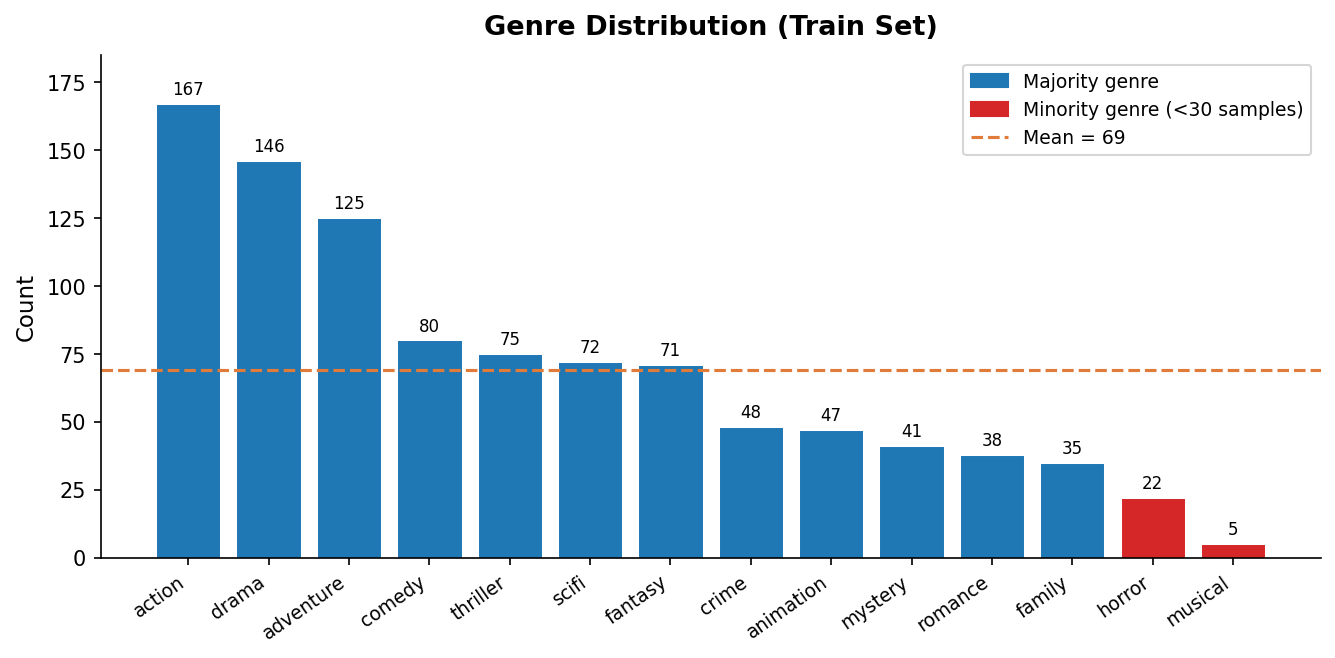
\includegraphics[width=\columnwidth]{genre_distribution.png}}
\caption{Genre distribution in the training set. Red bars indicate 
minority genres with fewer than 30 positive samples. The dashed line 
marks the mean count of 69.}
\label{fig:genre_dist}
\end{figure}

\subsection{Label Co-occurrence}

Figure~\ref{fig:cooc} presents the normalized genre co-occurrence 
matrix computed over the training set. Each cell $(i, j)$ represents 
the fraction of films labeled with genre $i$ that also carry genre $j$.

Several strong co-occurrence patterns emerge. \textit{Sci-fi} films 
are overwhelmingly labeled as \textit{action} (0.93) and 
\textit{adventure} (0.81), reflecting the typical narrative structure 
of blockbuster science fiction. \textit{Animation} films co-occur 
heavily with \textit{adventure} (0.94) and \textit{family} (0.60), 
consistent with the family-friendly nature of animated features. 
\textit{Crime} films frequently co-occur with \textit{drama} (0.73) 
and \textit{thriller} (0.67), while \textit{thriller} strongly 
correlates with \textit{drama} (0.72) and \textit{action} (0.69).

These high inter-label correlations indicate that movie genres are 
\textbf{not independent}, and a classifier that exploits label 
dependencies may achieve higher accuracy than one that treats each 
label in isolation. While the current architecture uses independent 
sigmoid outputs per label, the co-occurrence patterns also provide 
a useful diagnostic for interpreting per-genre errors.

\begin{figure}[htbp]
\centerline{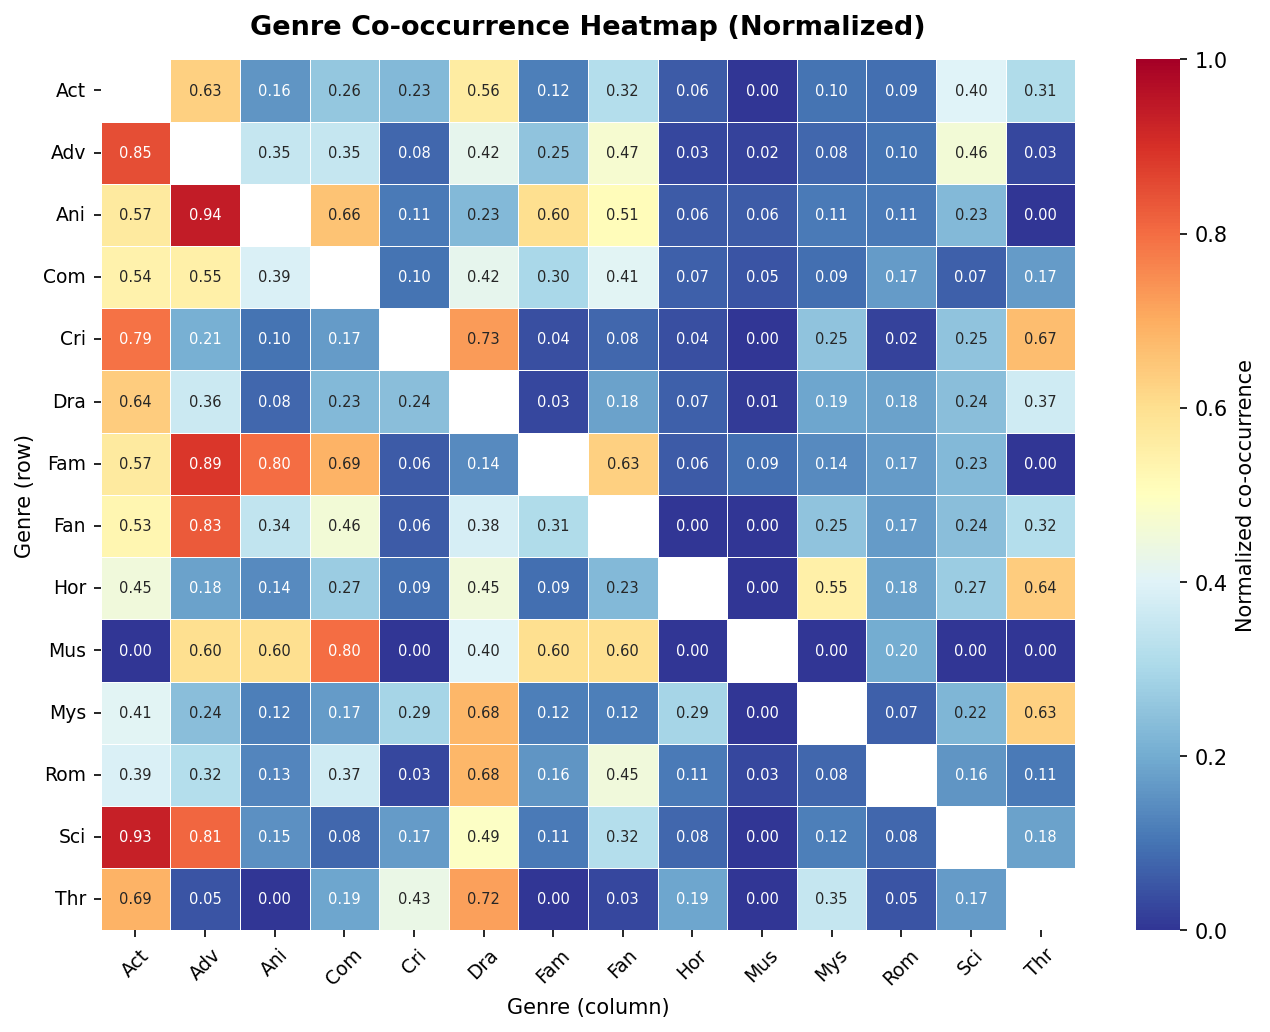
\includegraphics[width=\columnwidth]{cooccurrence_heatmap.png}}
\caption{Normalized genre co-occurrence heatmap over the training set.
Cell $(i,j)$ gives the fraction of genre-$i$ films that also belong 
to genre $j$. Abbreviations: Act=action, Adv=adventure, Ani=animation,
Com=comedy, Cri=crime, Dra=drama, Fam=family, Fan=fantasy, Hor=horror,
Mus=musical, Mys=mystery, Rom=romance, Sci=sci-fi, Thr=thriller.}
\label{fig:cooc}
\end{figure}

\subsection{Distribution of Genre Count per Film}

Figure~\ref{fig:genre_count} shows the distribution of the number of 
genre labels assigned to each film in the training and test sets. 
Both splits exhibit nearly identical distributions, with a mean of 
3.89 (train) and 3.86 (test) genres per film, confirming that the 
stratified split successfully preserves label-count statistics.

Almost no film in the dataset carries a single genre label; the vast 
majority of samples have between 3 and 5 co-occurring genres, with a 
peak at 4 labels (90 training samples, 23 test samples). This 
characteristic severely rules out single-label formulations and 
underscores the necessity of a multi-label approach with 
per-label binary cross-entropy loss.

\begin{figure}[htbp]
\centerline{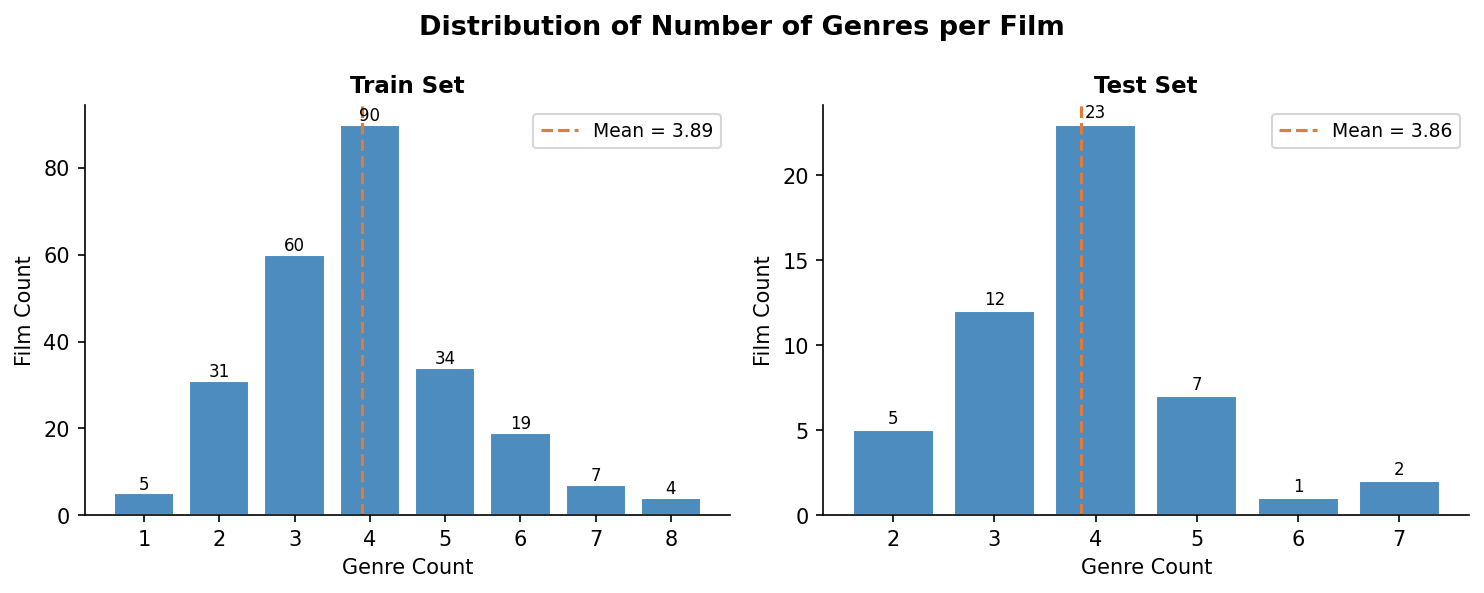
\includegraphics[width=\columnwidth]{genre_count_dist.png}}
\caption{Distribution of genre count per film for the training set 
(left) and test set (right). The dashed line marks the mean. Both 
splits peak at 4 genres per film, confirming consistent label-count 
distribution.}
\label{fig:genre_count}
\end{figure}

\subsection{Visual Feature Analysis: Brightness by Genre}

To examine whether low-level visual statistics differ meaningfully 
across genres, Figure~\ref{fig:brightness} presents the distribution 
of mean poster brightness (pixel intensity averaged over RGB channels, 
range 0--255) per genre.

A clear separation is visible at the extremes. \textit{Musical} posters 
are noticeably brighter overall, exhibiting a higher median brightness 
and a tighter, more elevated interquartile range relative to other 
genres. This is consistent with the typically colorful and vibrant 
visual language associated with musical productions. In contrast, 
\textit{horror}, \textit{crime}, and \textit{mystery} posters tend to 
be visually darker, with lower median brightness scores, reflecting 
their conventional use of dark color palettes and moody lighting to 
convey tension and unease.

These observations corroborate the hypothesis that genre-specific 
visual conventions are encoded in low-level poster statistics, 
motivating the use of a deep convolutional backbone capable of 
capturing both low-level (color, texture) and high-level (composition, 
semantic) visual features.

\begin{figure}[htbp]
\centerline{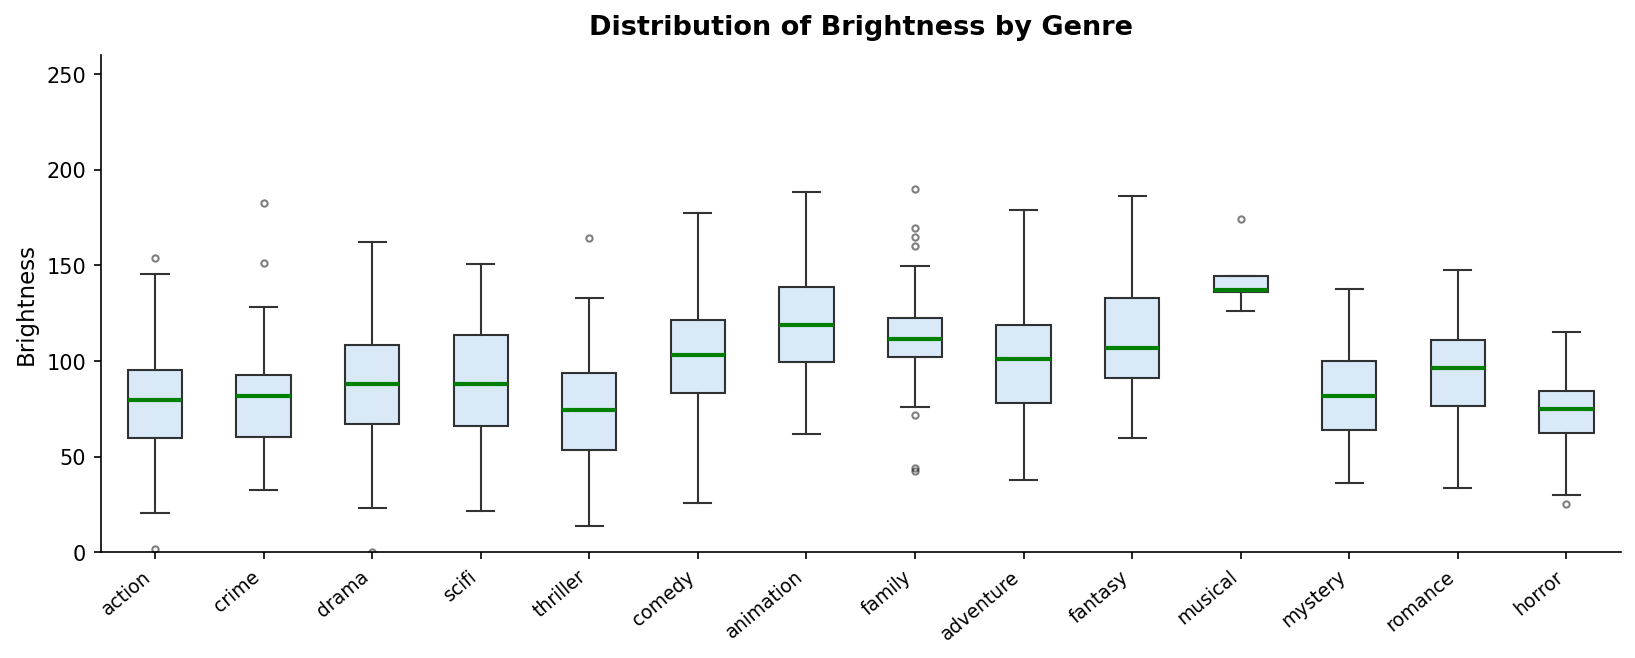
\includegraphics[width=\columnwidth]{brightness_by_genre.png}}
\caption{Distribution of mean poster brightness per genre.
Musicals display the highest median brightness, while horror, crime, 
and mystery genres are consistently darker, reflecting their 
genre-specific visual conventions.}
\label{fig:brightness}
\end{figure}

\subsection{Class Imbalance Analysis and Mitigation}

Table~\ref{tab:class_imbalance} summarizes the positive sample counts 
per genre across all splits. Three genres, \textit{musical} (5 
train), \textit{horror} (22 train), and \textit{romance} (38 train) 
--- fall below or near the minority threshold of 30 samples. Given 
the 80/20 train-validation split, the effective positive count 
available for gradient updates is even smaller after stratification.

\begin{table}[!t]
\caption{Positive Sample Count per Genre (Training Set)}
\label{tab:class_imbalance}
\begin{center}
\small
\begin{tabular}{lcc}
\hline
\textbf{Genre} & \textbf{Train Count} & \textbf{\% of Total Films} \\
\hline
Action      & 167 & 66.8\% \\
Drama       & 146 & 58.4\% \\
Adventure   & 125 & 50.0\% \\
Comedy      &  80 & 32.0\% \\
Thriller    &  75 & 30.0\% \\
Sci-fi      &  72 & 28.8\% \\
Fantasy     &  71 & 28.4\% \\
Crime       &  48 & 19.2\% \\
Animation   &  47 & 18.8\% \\
Mystery     &  41 & 16.4\% \\
Romance     &  38 & 15.2\% \\
Family      &  35 & 14.0\% \\
Horror      &  22 &  8.8\% \\
Musical     &   5 &  2.0\% \\
\hline
\textbf{Mean} & \textbf{69} & \textbf{27.6\%} \\
\hline
\end{tabular}
\end{center}
\end{table}

To partially mitigate the imbalance, two complementary strategies 
are employed. First, samples containing any genre with fewer than 
15 occurrences are duplicated five times in the training set 
(targeted oversampling), ensuring that minority-class gradients 
are amplified relative to the default data distribution. Second, 
per-class positive weights proportional to the negative-to-positive 
ratio (Eq.~\ref{eq:posweight}) are applied to the 
\texttt{BCEWithLogitsLoss}, penalizing false negatives on 
underrepresented genres more heavily than false negatives on 
majority genres. Despite these measures, the extremely low 
positive count of \textit{musical} (5 training samples) renders 
reliable classification practically infeasible, as confirmed by 
the zero F1-score on this genre in both experimental configurations 
(see Section~\ref{sec:results}).
% ============================================================
% ============================================================
\section{Methodology}
\label{sec:method}
% ============================================================
\subsection{Data Preprocessing}

\subsubsection{Image Preprocessing}
All poster images are resized to $300 \times 300$ pixels and normalized 
using ImageNet statistics ($\mu = [0.485, 0.456, 0.406]$, 
$\sigma = [0.229, 0.224, 0.225]$). Data augmentation is applied 
exclusively to the training split, as summarized in 
Table~\ref{tab:augmentation}.

\begin{table}[!t]
\caption{Image Augmentation Pipeline (Training Only)}
\label{tab:augmentation}
\begin{center}
\small
\begin{tabular}{lll}
\hline
\textbf{Transform} & \textbf{Parameter} & \textbf{Purpose} \\
\hline
RandomResizedCrop   & scale=(0.85,1.0)   & Crop variation  \\
RandomRotation      & degrees=5          & Light rotation  \\
ColorJitter         & brightness=0.10    & Color variation \\
GaussianBlur        & kernel=3, p=0.2    & Blur simulation \\
RandHorizontalFlip  & p=0.5              & Symmetry flip   \\
Normalize           & ImageNet stats     & Normalization   \\
\hline
\end{tabular}
\end{center}
\end{table}

\subsubsection{Text Preprocessing (Experiment I Only)}
Movie titles are tokenized using \texttt{BertTokenizer} from 
\texttt{bert-base-uncased} with \texttt{max\_length=16}, padding, 
and truncation enabled. The tokenizer produces \texttt{input\_ids} 
and \texttt{attention\_mask} as inputs to BERT.

\subsection{Model Architecture}

Two experimental configurations are evaluated, both using 
EfficientNet-B3 as the visual backbone.

\subsubsection{Experiment I: Multimodal EfficientNet-B3 + BERT + 
Cross-Attention}


The multimodal model processes two parallel streams. The visual stream 
passes the poster through EfficientNet-B3 (ImageNet pretrained), 
producing a 1536-d feature via \texttt{AdaptiveAvgPool2d(1)}, projected 
to 768-d via a linear layer. The textual stream encodes the movie title 
through \texttt{BERT-base-uncased}, averaging the last four layers' 
\texttt{[CLS]} tokens to produce a 768-d embedding.

The two embeddings are fused via an 8-head cross-attention mechanism, 
where the text embedding is the query and the projected image embedding 
provides keys and values. The cross-attended output is layer-normalized 
and concatenated with the original text and image embeddings, yielding 
a $768 + 768 + 768 = 2304$-d fused vector fed into the classifier head. 
The full component breakdown is shown in Table~\ref{tab:arch_exp1}.

\begin{table}[!t]
\caption{Model Components, Experiment I (Multimodal)}
\label{tab:arch_exp1}
\begin{center}
\small
\begin{tabular}{lp{3.2cm}c}
\hline
\textbf{Component} & \textbf{Detail} & \textbf{Dim} \\
\hline
\texttt{bert}            & BertModel, last 4 CLS avg        & 768  \\
\texttt{eff\_features}   & EfficientNetB3 conv trunk        & 1536 \\
\texttt{eff\_avgpool}    & AdaptiveAvgPool2d(1)             & 1536 \\
\texttt{img\_proj}       & Linear(1536, 768)                & 768  \\
\texttt{cross\_attn}     & MultiheadAttn(768, heads=8)      & 768  \\
\texttt{layer\_norm}     & LayerNorm(768)                   & 768  \\
\texttt{classifier[0]}   & Linear(2304, 1024)               & 1024 \\
\texttt{classifier[1-3]} & LayerNorm, ReLU, Dropout(0.3)   & 1024 \\
\texttt{classifier[4]}   & Linear(1024, 14)                 & 14   \\
\hline
\multicolumn{2}{l}{Total parameters (est.)} & $\pm$124M \\
\hline
\end{tabular}
\end{center}
\end{table}

\FloatBarrier
% Uncomment dan ganti nama file setelah diagram dibuat
\begin{figure}[!htbp]
\centerline{\includegraphics[width=0.8\columnwidth]{arch1.png}}
\caption{Architecture of Experiment I: EfficientNet-B3 + BERT + 
         Cross-Attention Fusion.}
\label{fig:arch_multi}
\end{figure}

\subsubsection{Experiment II: Image-Only EfficientNet-B3}


The image-only baseline passes the 1536-d EfficientNet-B3 feature 
directly to a two-layer classifier without any text input or fusion, 
as detailed in Table~\ref{tab:arch_exp2}. This configuration is kept
intentionally compact so that any performance difference can be
attributed to the added title-aware fusion path rather than to an
uncontrolled change in the visual backbone.

\begin{table}[!t]
\caption{Model Components, Experiment II (Image-Only)}
\label{tab:arch_exp2}
\begin{center}
\small
\begin{tabular}{lp{3.2cm}c}
\hline
\textbf{Component} & \textbf{Detail} & \textbf{Dim} \\
\hline
\texttt{backbone}        & EfficientNetB3 + AvgPool        & 1536 \\
\texttt{classifier[0]}   & Linear(1536, 512)               & 512  \\
\texttt{classifier[1-3]} & LayerNorm, ReLU, Dropout(0.3)  & 512  \\
\texttt{classifier[4]}   & Linear(512, 14)                 & 14   \\
\hline
\multicolumn{2}{l}{Total parameters (est.)} & $\pm$10.7M \\
\hline
\end{tabular}
\end{center}
\end{table}

\begin{figure}[!htbp]
\centerline{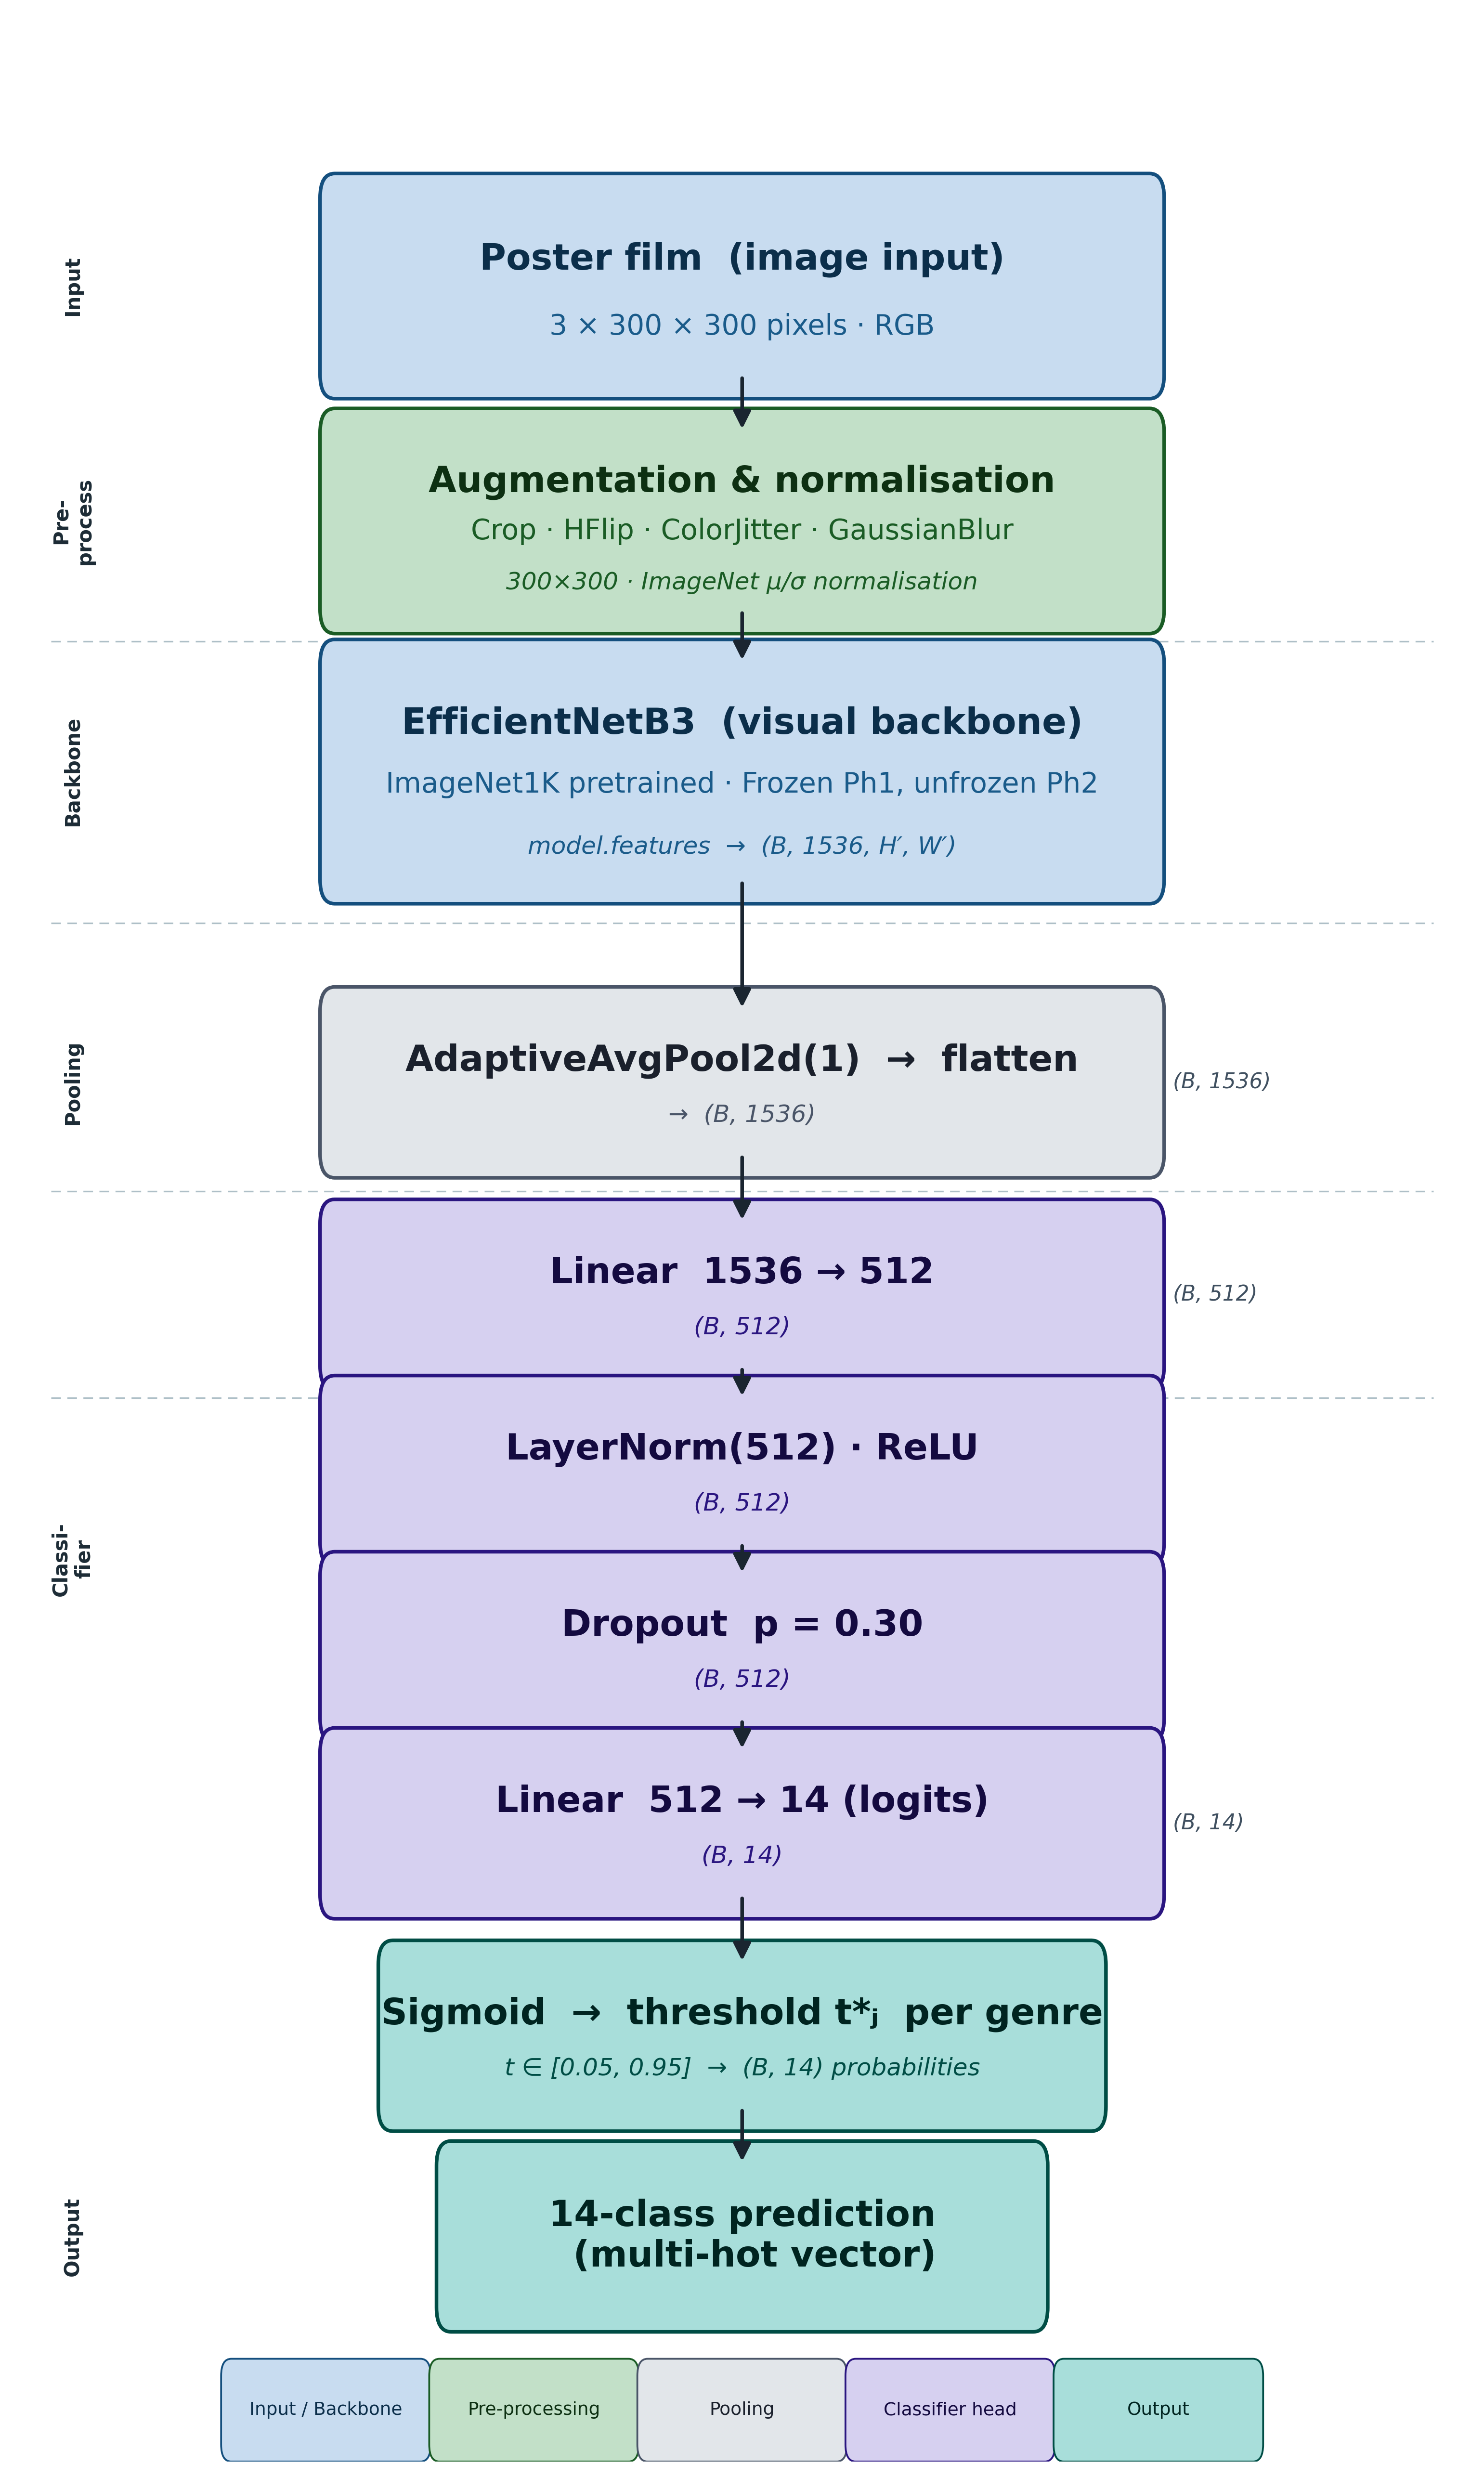
\includegraphics[width=0.8\columnwidth]{arch2.png}}
\caption{Architecture of Experiment II: EfficientNet-B3 Image-Only.}
\label{fig:arch_img}
\end{figure}

\FloatBarrier
\subsection{Experiment Setup}

\subsubsection{Data Strategy}

\paragraph{Train/Validation/Test Split.}
The dataset is split using \texttt{MultilabelStratifiedShuffleSplit} 
(80\% train / 20\% validation, random state 42), preserving multilabel 
distribution across splits. The held-out test set is used solely for 
final evaluation.

\paragraph{Targeted Oversampling.}
Samples containing any genre with fewer than 15 occurrences are 
duplicated $\times$5 on the training set only, preventing data leakage 
into validation and test sets.

\paragraph{Positive Weight.}
Per-class positive weights are applied to the loss to penalize 
false negatives on minority genres:
\begin{equation}
  w_i = \frac{N - n_i^+}{n_i^+ + \varepsilon}, \quad \varepsilon = 10^{-5}
  \label{eq:posweight}
\end{equation}
where $N$ is the total training samples and $n_i^+$ is the positive 
sample count for genre $i$.

\subsubsection{Loss Function}

\texttt{BCEWithLogitsLoss} with per-class positive weights is used 
as the primary loss function:
\begin{equation}
  \mathcal{L} = -\frac{1}{N \cdot C} \sum_{i=1}^{N} \sum_{j=1}^{C}
  \bigl[ w_j y_{ij} \log \sigma(z_{ij}) 
       + (1{-}y_{ij}) \log (1{-}\sigma(z_{ij})) \bigr]
  \label{eq:bce}
\end{equation}
where $y_{ij} \in \{0,1\}$ is the ground-truth label, $z_{ij}$ is 
the raw logit, and $\sigma(\cdot)$ is the sigmoid function. 
Asymmetric Loss (ASL) is also implemented as an alternative.

\subsubsection{Two-Phase Training}

Training is conducted in two phases to prevent catastrophic forgetting.

\textit{Phase 1 — Backbone Frozen (30 epochs):} The backbone is frozen 
in evaluation mode. Only the head (and fusion modules in Experiment I) 
are trained using \texttt{CosineAnnealingLR}:
\begin{equation}
  \eta(t) = \eta_{\min} + \frac{1}{2}(\eta_0 - \eta_{\min})
  \Bigl(1 + \cos\frac{\pi t}{T_{\max}}\Bigr)
  \label{eq:cosine}
\end{equation}
with $\eta_0 = 5{\times}10^{-4}$, $\eta_{\min} = 10^{-6}$, 
$T_{\max} = 30$.

\textit{Phase 2 — Full Fine-Tuning (60 epochs):} All parameters are 
unfrozen from the best Phase 1 checkpoint. Differential learning rates 
are applied: backbone at $10^{-5}$ and head/fusion at $5{\times}10^{-5}$ 
(ratio of 5$\times$). \texttt{OneCycleLR} is used per step with 15\% 
warm-up and cosine decay.

The complete hyperparameter configuration is listed in 
Table~\ref{tab:hyperparam}.

\begin{table}[!t]
\caption{Complete Hyperparameter Configuration}
\label{tab:hyperparam}
\begin{center}
\small
\begin{tabular}{lll}
\hline
\textbf{Parameter} & \textbf{Value} & \textbf{Exp.} \\
\hline
val\_ratio              & 0.2                & I, II \\
minority\_threshold     & 15                 & I, II \\
oversample\_factor      & 5                  & I, II \\
batch\_size             & 16                 & I, II \\
image\_size             & 300                & I, II \\
bert\_name              & bert-base-uncased  & I \\
max\_text\_len          & 16                 & I \\
epochs (Ph.1 / Ph.2)    & 30 / 60            & I, II \\
lr\_phase1              & $5\times10^{-4}$   & I, II \\
lr\_backbone            & $10^{-5}$          & I, II \\
lr\_classifier          & $5\times10^{-5}$   & I, II \\
weight\_decay           & 0.01               & I, II \\
dropout                 & 0.3                & I, II \\
Scheduler Ph.1          & CosineAnnealingLR  & I, II \\
Scheduler Ph.2          & OneCycleLR         & I, II \\
\hline
\end{tabular}
\end{center}
\end{table}

\subsubsection{Threshold Tuning Per-Genre}

The decision threshold is independently optimized per genre on the 
validation set by sweeping $t \in [0.05, 0.95]$ with step 0.01 and 
selecting $t_j^{*} = \arg\max_t\, \text{F1}(y_j, \hat{y}_j(t))$. 
The optimized thresholds are then applied during test set evaluation.

\subsubsection{Test-Time Augmentation}

To improve prediction robustness, $K{=}5$ augmented views per image 
are averaged at inference:
\begin{equation}
  \bar{p}_j = \frac{1}{K}\sum_{k=1}^{K} p_j^{(k)}, \quad K = 5
  \label{eq:tta}
\end{equation}

\subsection{Evaluation Metrics}

\paragraph{Macro F1-Score (primary).}
\begin{equation}
  \text{F1}_{\text{macro}} = \frac{1}{C}\sum_{j=1}^{C} \text{F1}_j
  \label{eq:f1macro}
\end{equation}
Treats all genres equally regardless of frequency, making it suitable 
for imbalanced multilabel evaluation.

\paragraph{Micro F1-Score (secondary).} Aggregates TP, FP, FN across 
all genres before computing F1, giving more weight to frequent genres.

\paragraph{Hamming Loss.}
\begin{equation}
  \mathcal{L}_{\text{Hamming}} = \frac{1}{N \cdot C}
  \sum_{i=1}^{N}\sum_{j=1}^{C} \mathbf{1}[\hat{y}_{ij} \neq y_{ij}]
  \label{eq:hamming}
\end{equation}

\paragraph{AUC-ROC.} Macro-averaged area under the ROC curve, computed 
per genre to assess ranking performance independent of threshold.

% ============================================================
% ============================================================
% ============================================================
\section{Results and Discussion}
\label{sec:results}
% ============================================================

\subsection{Quantitative Results}

Table~\ref{tab:results_main} presents the overall performance of both
experimental configurations on the held-out test set. For each model,
two evaluation scenarios are reported: a uniform threshold of
$t = 0.5$ applied identically to all genres, and per-genre optimized
thresholds obtained through F1-score maximization on the validation set
($t \in [0.05, 0.95]$, step $0.01$).

The results reveal a substantial and consistent performance gap between
the two architectures. At the default threshold of $t = 0.5$, the
multimodal model (Experiment~I) achieves a Macro~F1 of $0.6502$,
compared to only $0.4554$ for the image-only baseline
(Experiment~II), a margin of $+0.1948$. This gap persists after
per-genre threshold optimization, with Experiment~I reaching a
Macro~F1 of $0.7293$ against $0.5269$ for Experiment~II, confirming
that the multimodal advantage is robust and not an artifact of
threshold calibration.

Beyond Macro~F1, the multimodal model demonstrates consistently
superior behavior across all reported metrics at the default threshold.
It achieves a Micro~F1 of $0.8385$ versus $0.5598$ for the
image-only model, a Weighted~F1 of $0.8222$ versus $0.6381$, and a
dramatically lower Hamming Loss of $0.0814$ compared to $0.3257$.
The Exact Match Ratio of $56.00\%$ for Experiment~I versus $0.00\%$
for Experiment~II is particularly striking: the image-only baseline
fails to produce a single fully correct multilabel prediction on the
test set at the default threshold, suggesting that without title
context, the model's per-genre confidence scores are poorly calibrated
for the joint multilabel decision boundary.

After threshold optimization, the image-only model achieves an
Exact Match Ratio of $0.00\%$ and a Hamming Loss of $0.3400$, both
of which are worse than the multimodal model at the same setting
($0.30$, $0.0957$). This highlights that threshold tuning yields
a selective gain for Experiment~II, improving Macro~F1 by $+0.0715$
by recovering minority-class predictions, but cannot overcome the
underlying weakness in raw feature discrimination.

Notably, threshold optimization provides a larger relative gain for
Experiment~II ($+0.0715$ Macro~F1) than for Experiment~I ($+0.0791$),
but the absolute scores remain in favor of the multimodal model across
all thresholds. The consistent superiority of Experiment~I across all
metrics strongly supports the hypothesis that title-based textual
context provides complementary and discriminative information that
poster visual features alone cannot replicate.

\begin{table}[!t]
\caption{Overall Performance on Test Set}
\label{tab:results_main}

\centering
\footnotesize
\setlength{\tabcolsep}{3pt}
\renewcommand{\arraystretch}{1.1}

\resizebox{\columnwidth}{!}{%
\begin{tabular}{llccccc}
\hline
\textbf{Model} & \textbf{Thr.}
& \textbf{Macro F1} & \textbf{Micro F1}
& \textbf{Weighted F1}
& \textbf{Hamming}
& \textbf{Exact Match} \\
\hline

Exp.\ I (Multimodal)
& 0.5
& 0.6502
& 0.8385
& 0.8222
& 0.0814
& 56.00\% \\

Exp.\ I (Multimodal)
& optimal
& 0.7293
& 0.8393
& 0.8837
& 0.0957
& 30.00\% \\


Exp.\ II (Image-Only)
& 0.5
& 0.4554
& 0.5598
& 0.6381
& 0.3257
& 0.00\% \\

Exp.\ II (Image-Only)
& optimal
& 0.5269
& 0.5810
& 0.7055
& 0.3400
& 0.00\% \\

\hline
\end{tabular}%
}
\end{table}

\subsection{Per-Genre Analysis}

Table~\ref{tab:threshold_comparison} reports the per-genre F1 scores
for both models at the default ($t = 0.5$) and per-genre optimal
thresholds, alongside the optimal threshold $t^{*}_{j}$ selected for
each genre on the validation set.

\begin{table*}[!t]
\caption{Per-Genre F1 Comparison Before and After Threshold Optimization for Experiment I (Multimodal) and Experiment II (Image-Only)}
\label{tab:threshold_comparison}
\begin{center}
\small
\renewcommand{\arraystretch}{1.10}
\setlength{\tabcolsep}{4.5pt}

\begin{tabular}{l c c c c c c}
\hline

& \multicolumn{3}{c}{\textbf{Exp.\ I, Multimodal}}
& \multicolumn{3}{c}{\textbf{Exp.\ II, Image-Only}} \\

\cline{2-4} \cline{5-7}

\textbf{Genre}
& \textbf{$t^{*}$}
& \textbf{F1 @ 0.50}
& \textbf{F1 @ Optimal}

& \textbf{$t^{*}$}
& \textbf{F1 @ 0.50}
& \textbf{F1 @ Optimal} \\

\hline

Action
& 0.15 & 0.8986 & 0.9351
& 0.05 & 0.7895 & 0.8372 \\

Adventure
& 0.38 & 0.9767 & 0.9778
& 0.44 & 0.7308 & 0.7556 \\

Animation
& 0.29 & 0.8571 & 0.9333
& 0.60 & 0.7692 & 0.8571 \\

Comedy
& 0.47 & 0.7000 & 0.9231
& 0.39 & 0.5116 & 0.6452 \\

Crime
& 0.13 & 0.6667 & 0.7857
& 0.32 & 0.4400 & 0.4681 \\

Drama
& 0.39 & 0.9714 & 0.9855
& 0.45 & 0.8608 & 0.8684 \\

Family
& 0.89 & 0.3333 & 0.4000
& 0.81 & 0.2857 & 0.3333 \\

Fantasy
& 0.76 & 0.7368 & 0.7619
& 0.37 & 0.4138 & 0.5000 \\

Horror
& 0.78 & 0.8000 & 1.0000
& 0.40 & 0.0909 & 0.1429 \\

Musical
& 0.05 & 0.0000 & 0.0000
& 0.05 & 0.0000 & 0.0000 \\

Mystery
& 0.10 & 0.4444 & 0.6207
& 0.36 & 0.4324 & 0.4898 \\

Romance
& 0.06 & 0.0000 & 0.0870
& 0.23 & 0.0000 & 0.0556 \\

Sci-fi
& 0.68 & 0.9286 & 0.9630
& 0.60 & 0.4000 & 0.7200 \\

Thriller
& 0.31 & 0.7895 & 0.8372
& 0.45 & 0.6512 & 0.7037 \\

\hline

\textbf{Macro F1}
& \textbf{0.39}
& \textbf{0.6502}
& \textbf{0.7293}

& \textbf{0.39}
& \textbf{0.4554}
& \textbf{0.5269} \\

\hline
\end{tabular}

\end{center}

\vspace{2pt}

{\footnotesize
Note: $t^{*}$ denotes the optimal decision threshold selected independently for each genre based on validation F1-score maximization.
}

\end{table*}

\begin{figure}[!t]
\centerline{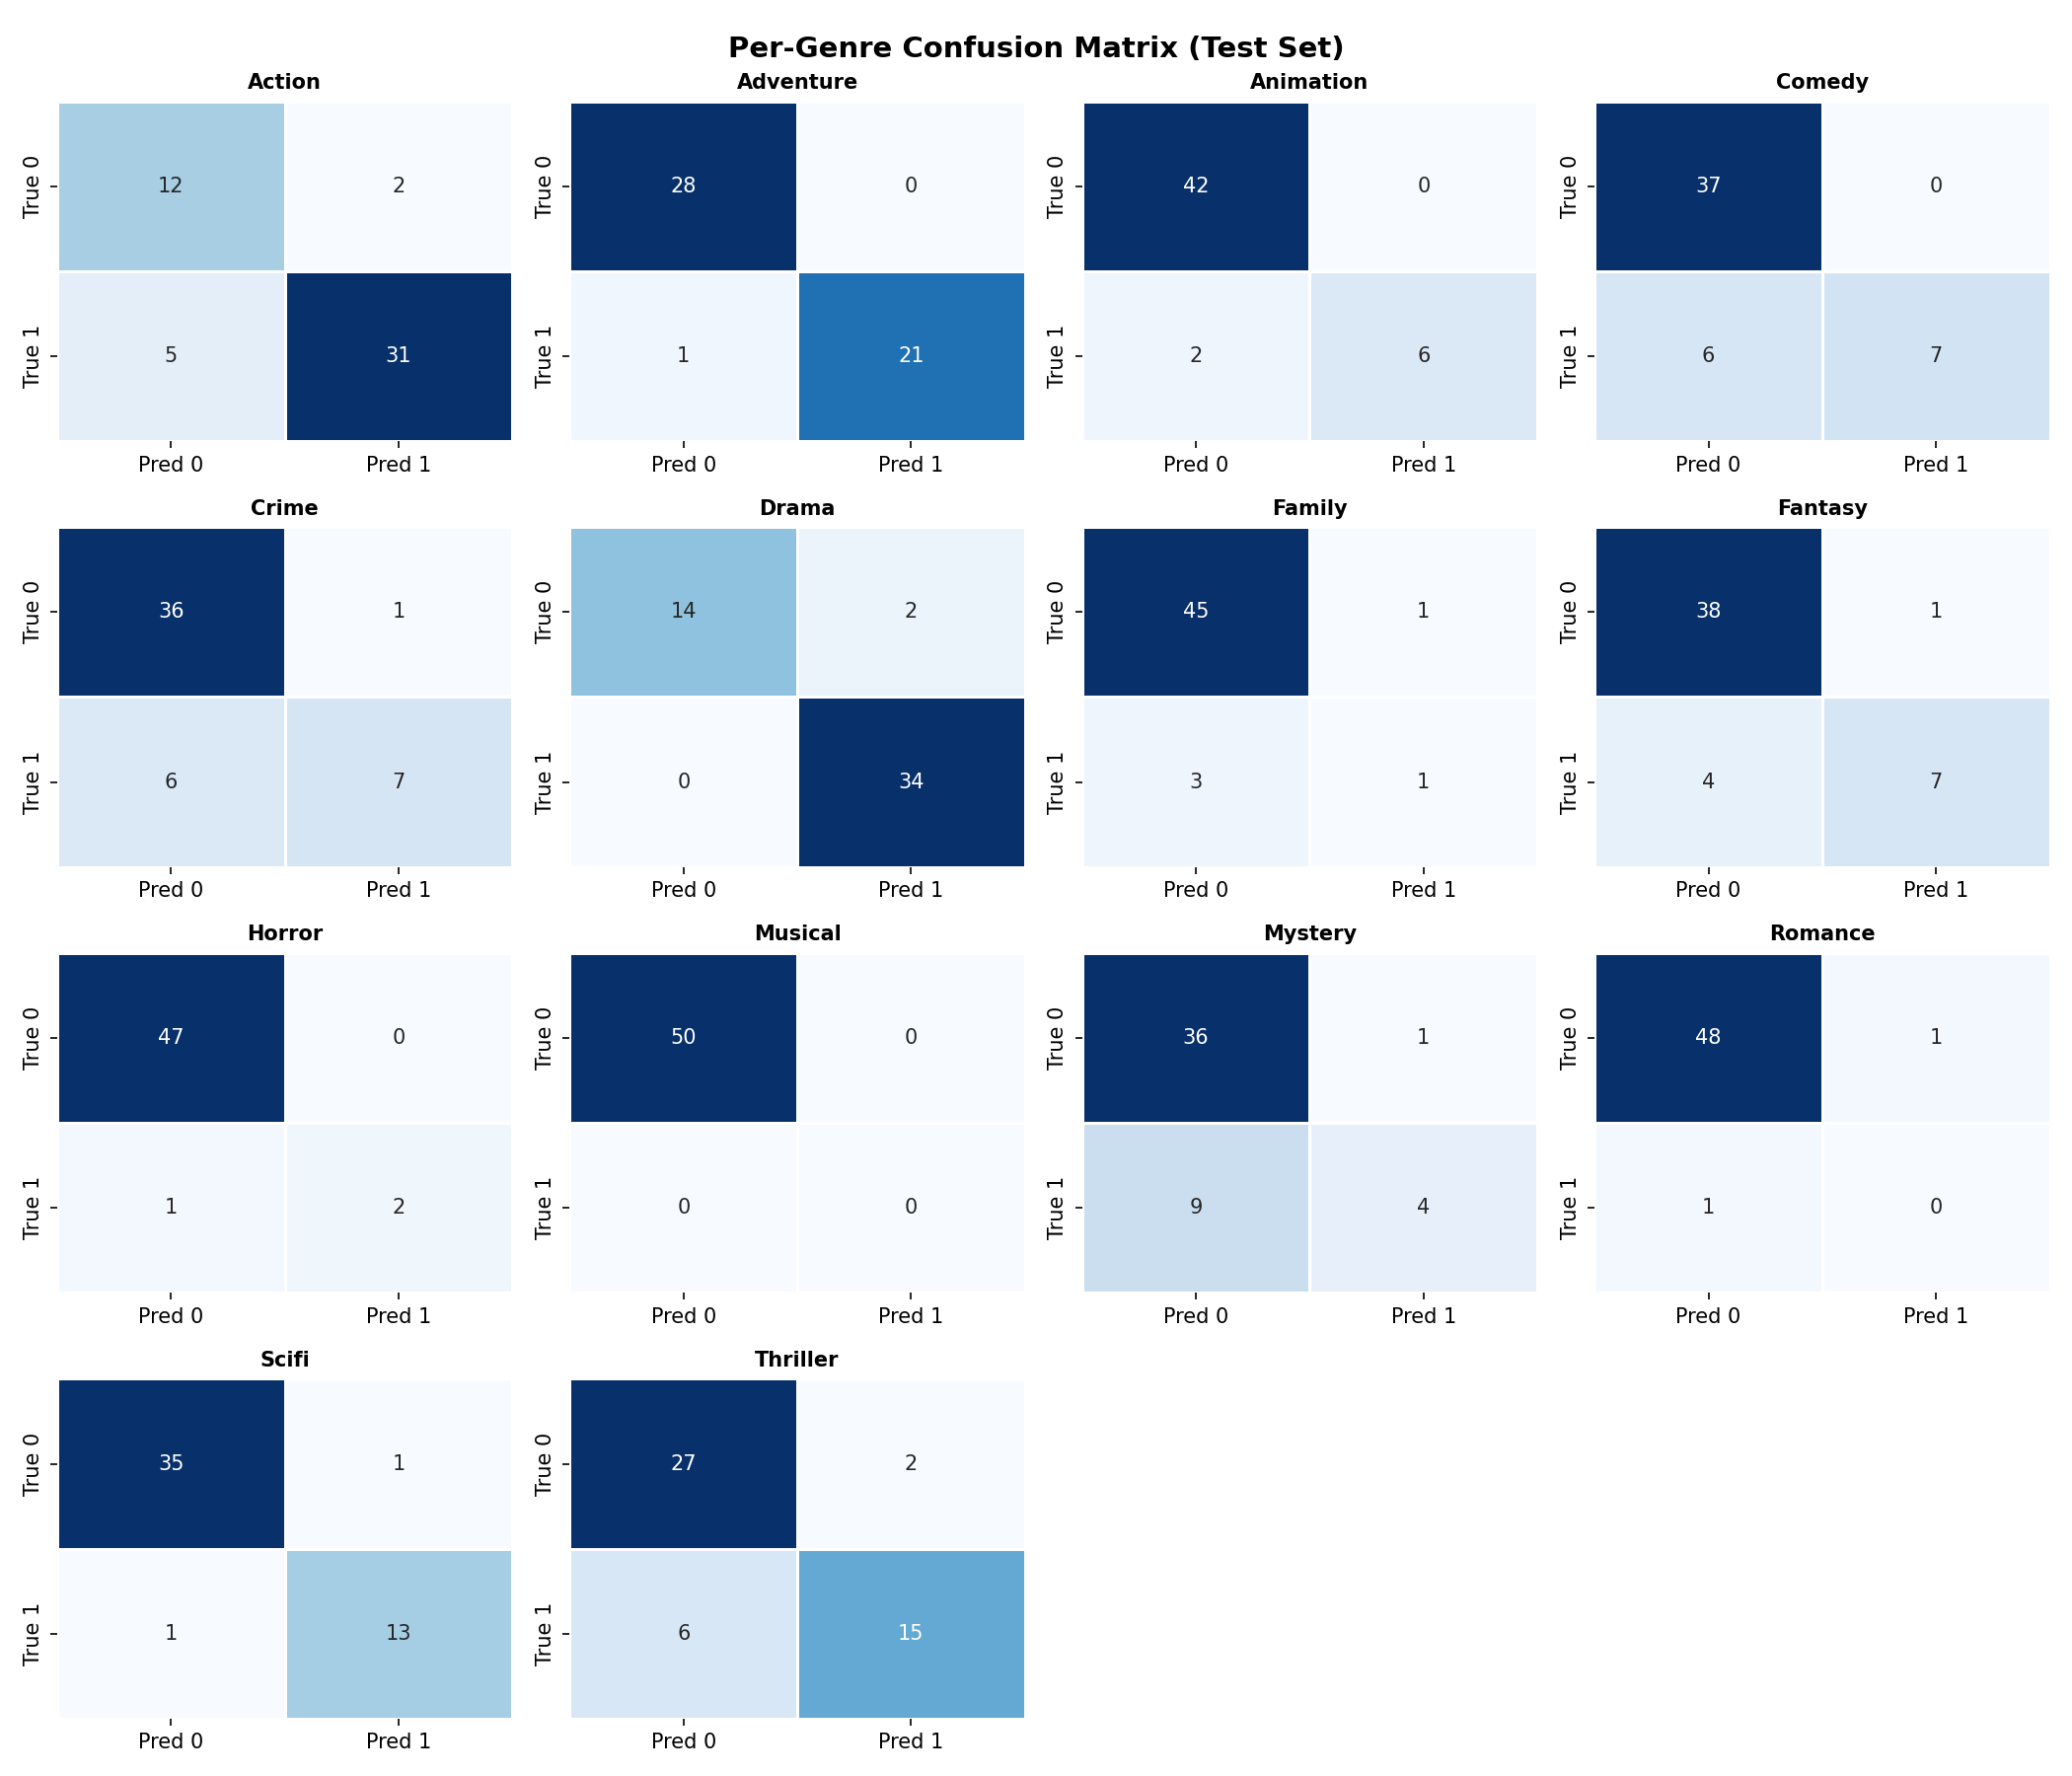
\includegraphics[width=\columnwidth]{cm_exp1.png}}
\caption{Per-genre confusion matrices, Experiment~I (Multimodal).
         Each $2{\times}2$ matrix shows TN/FP/FN/TP counts on the
         test set at the per-genre optimal threshold.}
\label{fig:cm_exp1}
\end{figure}

\begin{figure}[!t]
\centerline{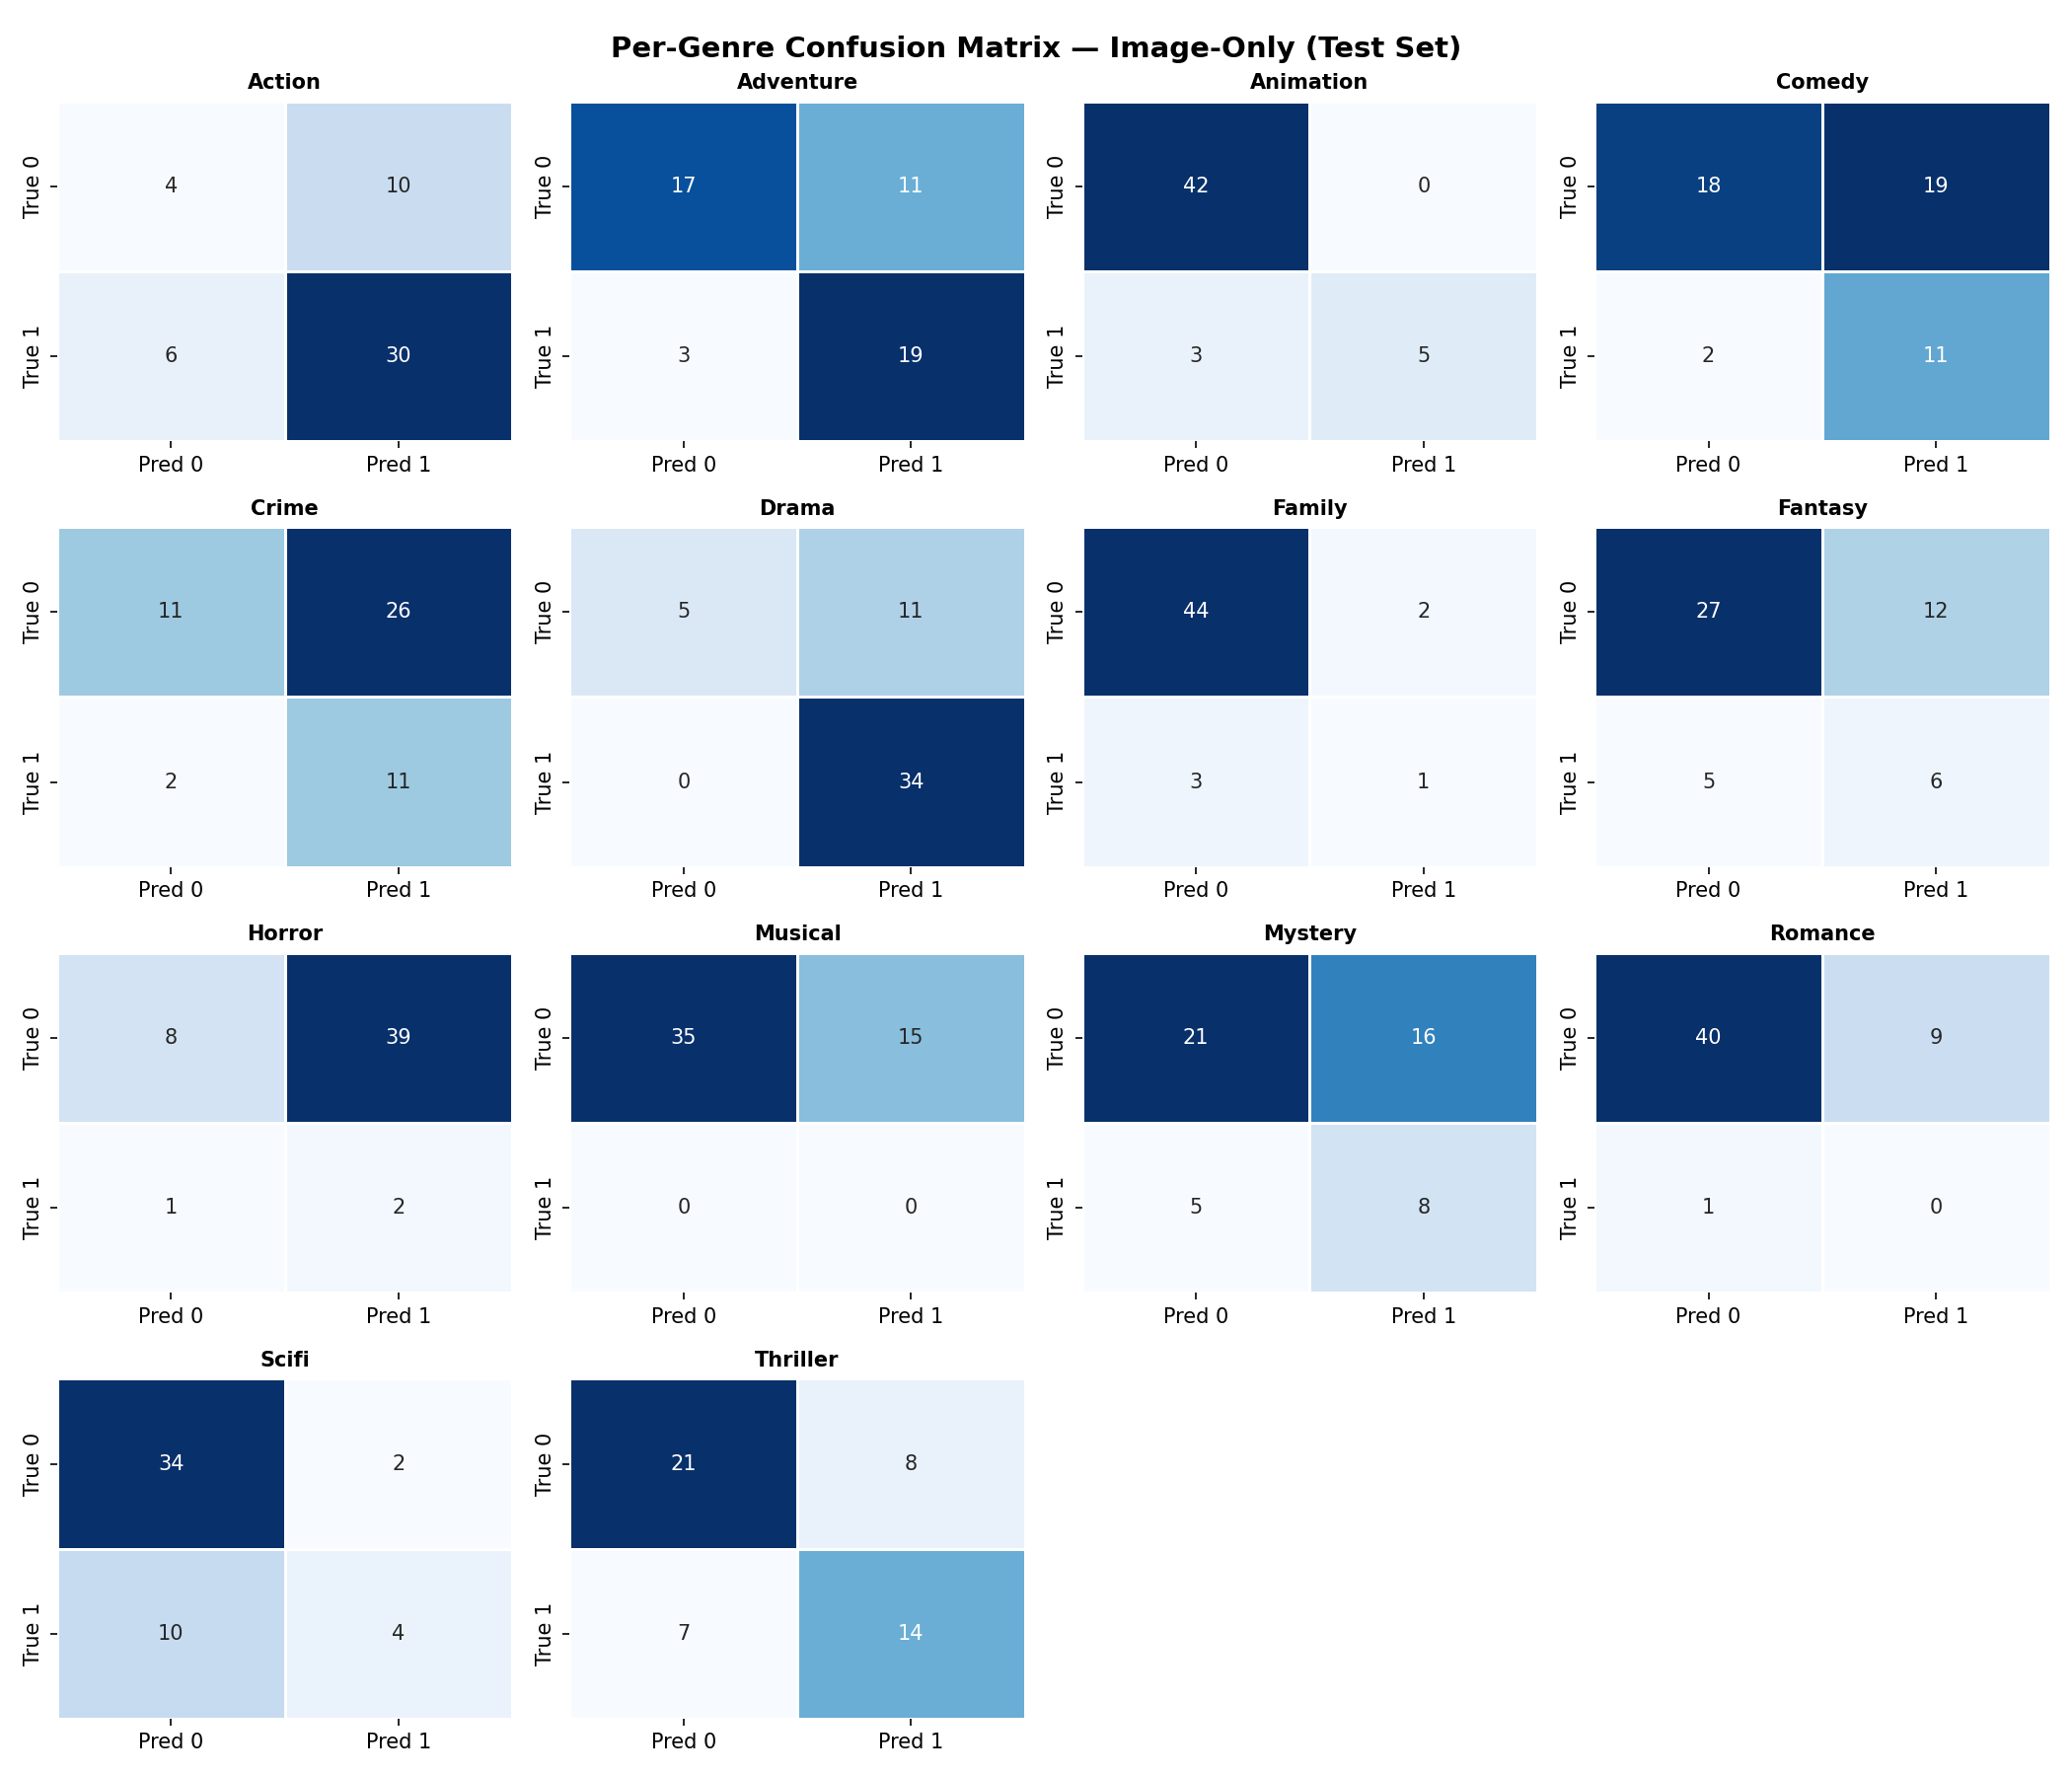
\includegraphics[width=\columnwidth]{cm_exp2.png}}
\caption{Per-genre confusion matrices, Experiment~II (Image-Only).}
\label{fig:cm_exp2}
\end{figure}

Several observations emerge from the per-genre analysis.

\subsubsection{Genres with Zero or Near-Zero Test Positives}

Both models completely fail on \textit{musical} (F1 $= 0.00$) and
\textit{romance} (F1 $\leq 0.09$) regardless of architecture or
threshold strategy. Inspection of the confusion matrices confirms
this: for \textit{musical}, Experiment~I (Fig.~\ref{fig:cm_exp1})
shows 50~TN and 0~TP, with all test instances falling into the
negative class, meaning there are zero positive test samples for
this genre. For \textit{romance}, only 1 positive test sample exists,
and it is misclassified as a negative by both models.

These failures are a direct consequence of extreme class sparsity.
With only 5 training samples for \textit{musical} and 38 for
\textit{romance}, neither targeted oversampling nor positive-weight
BCE can compensate for the near-absence of a meaningful training
signal. This is a dataset-level limitation that no architectural
improvement can resolve.

\subsubsection{Title-Sensitive Genres}

The most pronounced gains for the multimodal model are observed on
genres that carry strong and consistent lexical signals in their titles.
\textit{Sci-fi} shows a dramatic improvement: at the default threshold,
Experiment~I achieves F1 $= 0.9286$ versus only $0.4000$ for
Experiment~II, with further improvement to $0.9630$ versus $0.7200$
after optimization. Similarly, \textit{horror} achieves F1 $= 0.8000$
versus $0.0909$ (at $t = 0.5$) and $1.0000$ versus $0.1429$ after
optimization, a near-perfect score for the multimodal model versus
near-complete failure for the image-only baseline.

Inspection of the confusion matrices supports these figures.
For \textit{horror}, Experiment~I (Fig.~\ref{fig:cm_exp1}) records
47~TN, 0~FP, 1~FN, and 2~TP at the optimal threshold, indicating
strong true-negative specificity with minimal false positives, while
Experiment~II (Fig.~\ref{fig:cm_exp2}) records 8~TN, 39~FP, 1~FN,
and 2~TP, a massive false-positive rate that severely degrades
precision. This pattern is consistent with the hypothesis that horror
posters may visually overlap with other dark-toned genres (crime,
thriller, mystery), but horror-specific title words provide the
disambiguation necessary for accurate classification.

\textit{Adventure} and \textit{fantasy} show similar patterns.
\textit{Adventure} reaches F1 $= 0.9778$ in Experiment~I versus
$0.7556$ in Experiment~II after optimization, while
\textit{fantasy} achieves $0.7619$ versus $0.5000$.
For \textit{sci-fi}, the confusion matrix of Experiment~II
(Fig.~\ref{fig:cm_exp2}) reveals 34~TN but 2~FP, 10~FN, and only
4~TP at the optimal threshold, demonstrating that the image-only
model fails to identify the majority of sci-fi positives, whereas
Experiment~I recovers 13~TP with only 1~FN and 1~FP
(Fig.~\ref{fig:cm_exp1}).

These observations are consistent with the findings of the
GradCAM analysis (Section~\ref{sec:gradcam}), which demonstrates
that the cross-attention mechanism guides EfficientNet-B3 to attend
to world-building background elements, spacecraft, cosmic
environments, supernatural settings, that are highly informative
for these genres when cued by the title embedding.

\subsubsection{Visually Dominant Genres}

For genres where visual cues are strong and consistent across posters,
both models perform comparably, and the multimodal advantage narrows.
\textit{Drama} achieves F1 $= 0.9855$ (Experiment~I) versus
$0.8684$ (Experiment~II) after optimization, both high, with the
gap attributable to the multimodal model's more precise threshold
selection ($t^{*} = 0.39$ vs.\ $0.45$). Confusion matrices confirm
that both models produce near-zero false negatives on drama
(Fig.~\ref{fig:cm_exp1} and Fig.~\ref{fig:cm_exp2}), reflecting
the genre's high frequency and visually diverse but still distinctive
poster characteristics (e.g., portrait compositions, muted palettes).

\textit{Animation} also shows comparable strong performance for both
models (F1 $= 0.9333$ vs.\ $0.8571$ after optimization), as
animation posters are visually distinctive with stylized character
designs and vivid color palettes that serve as robust visual
classifiers independently of title information.

\textit{Crime} and \textit{mystery}, while semantically related,
display a moderate multimodal advantage ($0.7857$ vs.\ $0.4681$ and
$0.6207$ vs.\ $0.4898$ respectively). The confusion matrix for
Experiment~II shows a high false-positive rate for crime
(Fig.~\ref{fig:cm_exp2}: 26~FP versus 1~FP in Experiment~I), likely
because crime poster aesthetics (dark tones, urban settings,
characters in formal attire) visually overlap with drama and
thriller.

\subsubsection{Genres with Low Overall Performance}

\textit{Family} remains a weak genre for both models despite its
moderate training count (35~samples). F1 scores of $0.4000$
(Experiment~I) and $0.3333$ (Experiment~II) after optimization
reflect its high visual variability: family-genre posters may
feature animated characters, live-action children's adventures, or
broad comedies, making them visually indistinct as a genre cluster.
Both confusion matrices show very few true positives (1 each),
indicating that the models overwhelmingly default to predicting
the negative class.

Taken together, the per-genre results indicate that the proposed
multimodal architecture is most beneficial when title semantics can
resolve visual ambiguity, while gains are smaller for categories that
are either already visually distinctive or too underrepresented to
provide reliable learning signals. This interpretation motivates the
training-dynamics analysis in the next subsection, which examines
whether the observed performance differences are supported by the
optimization behavior of both models.

\FloatBarrier
\subsection{Training Dynamics}
\label{sec:training_dynamics}

\subsubsection{Phase 1, Frozen Backbone}

Fig.~\ref{fig:loss_exp1_p1} and Fig.~\ref{fig:loss_exp2_p1} show
the Phase~1 training and validation loss curves for Experiments~I
and~II, respectively. Both models exhibit a characteristic divergence
pattern: training loss decreases sharply, converging to near zero
within the first 10~epochs, while validation loss increases
monotonically throughout all 30~epochs, rising from approximately
$0.85$ to $1.20$ (Experiment~I) and $1.15$ (Experiment~II).

This behavior is a direct consequence of the frozen-backbone
constraint: only the classifier head (and cross-attention fusion
module in Experiment~I) is optimized, while EfficientNet-B3
and BERT weights remain fixed. With the backbone unable to adapt
its representations to the dataset distribution, the trainable
classifier rapidly memorizes augmented training samples, a process
accelerated by the positive-weight BCE, which strongly penalizes
false negatives on minority classes and incentivizes high-confidence
positive predictions.

The divergence is more pronounced in Experiment~I than
Experiment~II. The multimodal model's larger trainable head
(encompassing the 8-head cross-attention, layer normalization, and
a $2304 \rightarrow 1024 \rightarrow 14$ classifier) provides
greater capacity for overfitting relative to the simpler
$1536 \rightarrow 512 \rightarrow 14$ head of the image-only model.
Nevertheless, the Phase~1 checkpoint serves its intended purpose:
it initializes the head with reasonable feature-to-label mappings
before the higher-risk full fine-tuning in Phase~2.

\begin{figure}[H]
\centerline{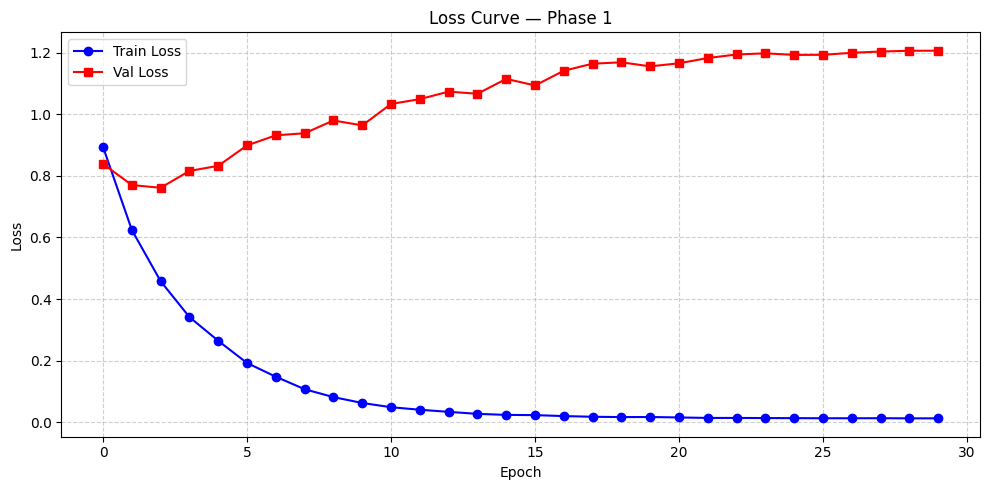
\includegraphics[width=0.92\columnwidth]{loss_exp1_p1.png}}
\caption{Loss curve, Phase~1, Experiment~I (Multimodal).}
\label{fig:loss_exp1_p1}
\end{figure}

\begin{figure}[H]
\centerline{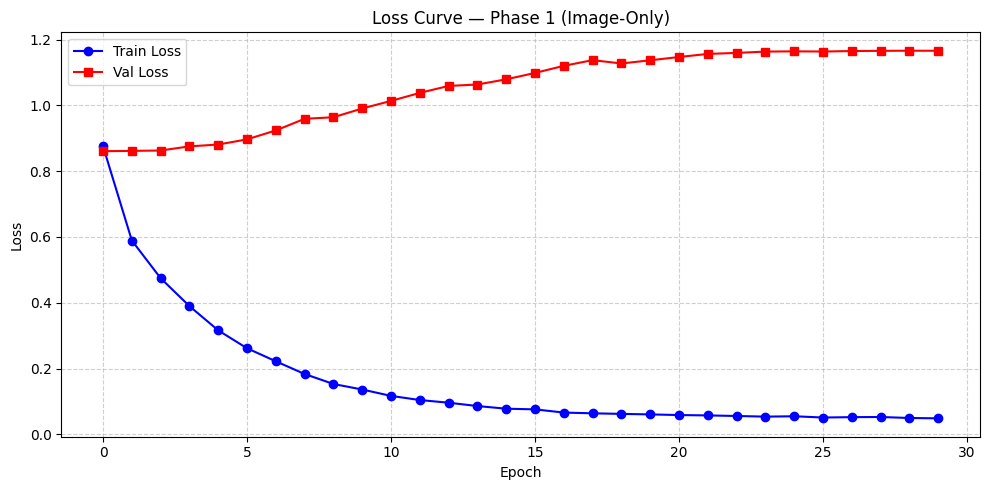
\includegraphics[width=0.92\columnwidth]{loss_exp2_p1.png}}
\caption{Loss curve, Phase~1, Experiment~II (Image-Only).}
\label{fig:loss_exp2_p1}
\end{figure}

\FloatBarrier
\subsubsection{Phase 2, Full Fine-Tuning}

The Phase~2 dynamics differ markedly between the two experiments,
as shown in Fig.~\ref{fig:loss_exp1_p2} and
Fig.~\ref{fig:loss_exp2_p2}.

For Experiment~II (image-only, Fig.~\ref{fig:loss_exp2_p2}),
Phase~2 exhibits a healthy and stable fine-tuning pattern.
Training loss decreases gradually from approximately $0.85$ to
$0.34$ over 60~epochs, following the smooth trajectory imposed by
\texttt{OneCycleLR}. Crucially, validation loss also decreases
initially, dropping from $\approx 0.90$ to $\approx 0.84$
within the first 5~epochs, before stabilizing around $0.86$
through the remainder of training. The absence of a significant
train-validation gap after epoch 10 indicates that EfficientNet-B3
fine-tuning successfully adapts the backbone's visual representations
to the poster domain while maintaining generalization. The
differential learning rate strategy (backbone at $10^{-5}$,
head at $5 \times 10^{-5}$) appears effective in preventing
catastrophic forgetting of ImageNet features while enabling
task-specific specialization.

For Experiment~I (multimodal, Fig.~\ref{fig:loss_exp1_p2}),
Phase~2 reveals a qualitatively different dynamic. Training loss
decreases steeply from $\approx 0.57$ to $\approx 0.07$ over
60~epochs, a substantially lower final training loss than
Experiment~II, while validation loss follows a trajectory with
an initial drop from $\approx 0.74$ to $\approx 0.53$ within the
first 15~epochs, followed by a plateau and stabilization around
$0.53$. Although the model does not exhibit catastrophic divergence,
the persistent and widening train-validation gap indicates that the
larger parameter space introduced by BERT ($\sim$110M parameters)
creates an overfitting pressure that the dataset of 250 training
samples cannot fully regularize. The weight decay of $0.01$ and
dropout of $0.3$ partially mitigate this, but they are insufficient
given the extreme model-to-data ratio.

This observation is consistent with the quantitative result that
threshold optimization yields a smaller macro-level gain for
Experiment~I: the model's sigmoid outputs for uncertain genres
reflect overconfident but poorly calibrated predictions,
which limits the benefit of per-genre threshold sweeping.

\begin{figure}[H]
\centerline{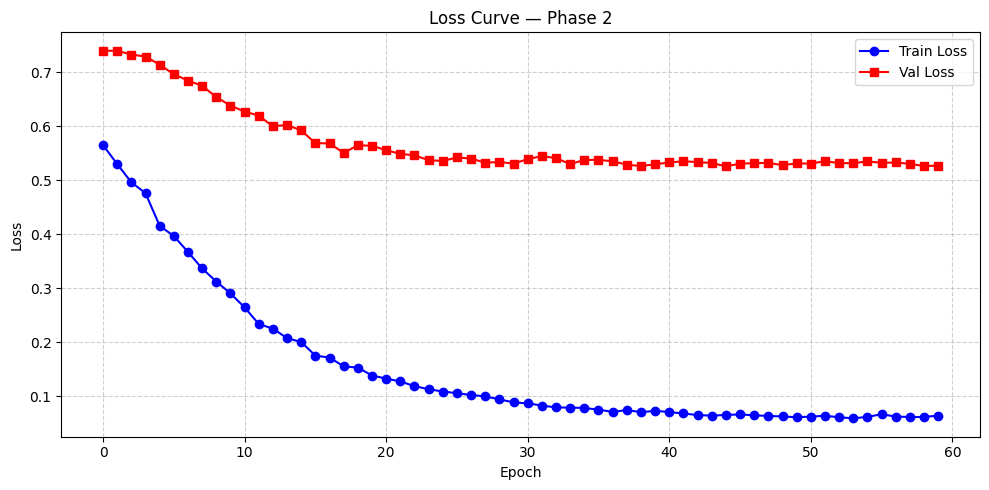
\includegraphics[width=0.92\columnwidth]{loss_exp1_p2.png}}
\caption{Loss curve, Phase~2, Experiment~I (Multimodal).}
\label{fig:loss_exp1_p2}
\end{figure}

\begin{figure}[H]
\centerline{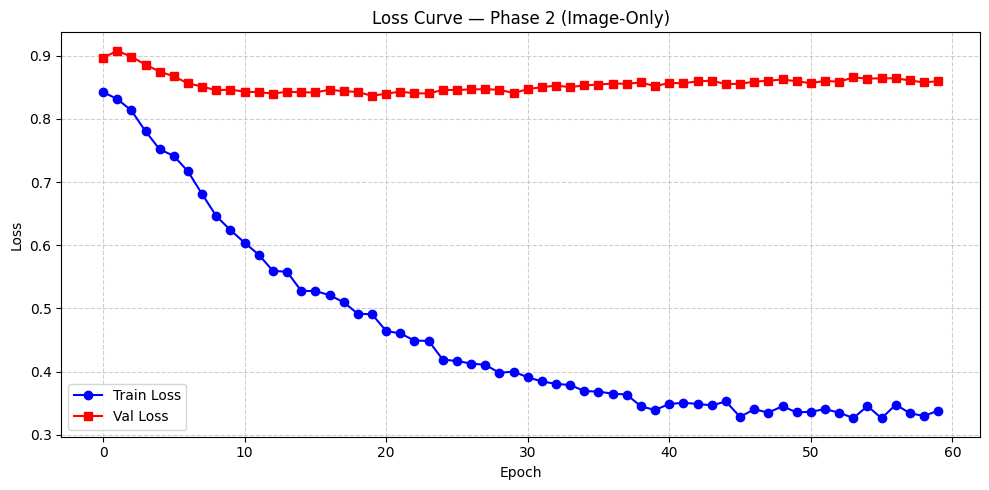
\includegraphics[width=0.92\columnwidth]{loss_exp2_p2.png}}
\caption{Loss curve, Phase~2, Experiment~II (Image-Only).}
\label{fig:loss_exp2_p2}
\end{figure}

\FloatBarrier
\subsection{Visual Explanation: GradCAM Analysis}
\label{sec:gradcam}

To qualitatively assess which spatial regions of the poster drive
genre predictions, Gradient-weighted Class Activation Mapping
(GradCAM)~\cite{gradcam} is applied to the final convolutional block
of EfficientNet-B3. Fig.~\ref{fig:gradcam_exp1} presents a
representative example from Experiment~I using the poster of
\textit{Guardians of the Galaxy} (true labels: action, adventure,
comedy, sci-fi).

\begin{figure}[!htbp]
\centerline{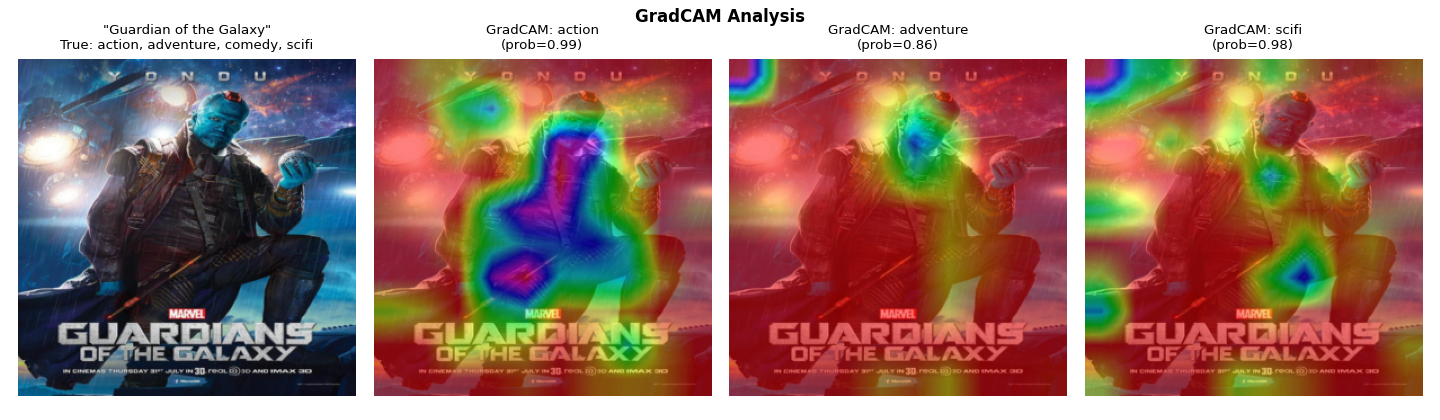
\includegraphics[width=\columnwidth]{gradcam_guardians.png}}
\caption{GradCAM visualizations for \textit{Guardians of the Galaxy}
         (Experiment~I, Multimodal). From left: original poster;
         activation map for \textit{action} (prob $= 0.99$),
         \textit{adventure} (prob $= 0.86$), and
         \textit{sci-fi} (prob $= 0.98$). Warmer colors indicate
         regions of higher gradient activation.}
\label{fig:gradcam_exp1}
\end{figure}

The GradCAM maps reveal that the model attends to semantically
meaningful and genre-discriminative spatial regions, with distinct
activation patterns for each predicted genre:

\begin{itemize}
  \item For \textbf{action} (prob $= 0.99$), the activation map
        shows intense concentration on the central humanoid figure,
        particularly the torso, arms, and weapon held in a combat-ready
        pose. Secondary activations appear at energy effects and
        dynamic foreground elements. This is consistent with
        action genre conventions, where powerful, kinetic character
        poses serve as the primary visual indicator. The model
        correctly ignores the background, which is shared with
        other genres.

  \item For \textbf{adventure} (prob $= 0.86$), the activation
        spreads more broadly across the figure and upper background,
        suggesting the model integrates multiple spatial cues,
        character silhouette, spacecraft visible in the upper left,
        and the expansive cosmic environment, rather than attending
        to a single focal point. This broader integration reflects the
        compositional nature of adventure genre posters, which
        typically communicate scope and journey through environmental
        context alongside character.

  \item For \textbf{sci-fi} (prob $= 0.98$), the activation
        pattern shifts notably toward the title region and the
        spacecraft and cosmic background in the upper portion of
        the poster. The reduced character-centered activation and
        increased attention to world-building background elements
        indicates that sci-fi classification relies on contextual
        cues such as futuristic technology and deep-space environments
        rather than character pose alone. This shift is likely
        mediated by the cross-attention mechanism: the title
        embedding for ``Guardians of the Galaxy'' contains
        strong sci-fi lexical cues (``Galaxy'') that guide the
        visual attention toward cosmologically informative regions.
\end{itemize}

These attention patterns demonstrate that EfficientNet-B3's final
convolutional features learn spatially structured,
genre-discriminative representations. Importantly, the activation
differences between genres on the same poster confirm that the
model is not learning a single global feature vector, but rather
genre-specific spatial patterns, a property that the cross-attention
mechanism in Experiment~I can selectively amplify based on the title
embedding. The qualitative evidence from GradCAM thus provides
mechanistic support for the quantitative advantage of the multimodal
architecture on lexically distinctive genres such as sci-fi, horror,
and adventure.

\subsection{Threshold Optimization Analysis}

The optimal thresholds $t^{*}_{j}$ listed in
Table~\ref{tab:threshold_comparison} vary substantially across genres
and models, ranging from $0.05$ to $0.89$ for Experiment~I and
$0.05$ to $0.81$ for Experiment~II. This variability confirms that
a uniform threshold of $0.5$ is systematically suboptimal for
imbalanced multilabel settings.

A clear pattern emerges: minority genres with few positive test
instances tend to receive low optimal thresholds (e.g.,
\textit{musical}: $t^{*} = 0.05$; \textit{romance}: $0.06$ for
Experiment~I, $0.23$ for Experiment~II; \textit{crime}: $0.13$).
This reflects the model's conservative sigmoid outputs for
underrepresented classes, since positive-weight BCE incentivizes
recall, the model produces low-confidence positive scores for
minority genres, requiring a low decision boundary to recover any
true positives.

Conversely, visually or lexically unambiguous genres tend to have
higher optimal thresholds (\textit{family}: $0.89$;
\textit{fantasy}: $0.76$ for Experiment~I), indicating that the
model produces high-confidence positive predictions for these
genres but with poor precision, necessitating a higher threshold
to suppress false positives.

For Experiment~I, the macro-level gain from threshold optimization
($+0.0791$ Macro~F1) is driven primarily by improvements on
\textit{action} ($+0.0365$), \textit{animation} ($+0.0762$),
\textit{comedy} ($+0.2231$), \textit{crime} ($+0.1190$), and
\textit{sci-fi} ($+0.0344$). For Experiment~II, larger gains on
\textit{sci-fi} ($+0.3200$) and \textit{thriller} ($+0.0525$)
drive the overall improvement.

\subsection{Discussion}

The results highlight three principal findings.

\textit{Title information provides a large and consistent advantage.}\
The multimodal architecture achieves substantially higher performance
across all metrics and thresholds, with the gap most pronounced on
genres with strong lexical title cues. The cross-attention mechanism
enables selective exploitation of title semantics to guide visual
feature interpretation, resulting in more precise per-genre
predictions and better-calibrated sigmoid outputs. This confirms
that movie titles, despite being a lightweight and universally
available textual signal, encode genre-discriminative information
that complements visual poster features in a non-trivial way.

\textit{Class imbalance is the primary performance bottleneck.}\
The complete failure on \textit{musical} and near-failure on
\textit{romance} and \textit{family} underscores that severe
class imbalance, particularly genres with fewer than 5 positive
test samples, represents a fundamental limitation that no
architectural innovation can overcome without sufficient training
data. Targeted oversampling and positive-weight BCE reduce the
false-negative rate on these genres during training but cannot
generate new discriminative signal where none exists.

\textit{Model capacity must be matched to dataset size.}\
The Phase~1 overfitting pattern and the persistent
train-validation gap in Phase~2 of Experiment~I illustrate the
mismatch between the $\sim$124M-parameter multimodal model and a
dataset of 250 training samples. While the multimodal model
ultimately outperforms the image-only baseline, indicating that
the additional parameters do carry useful inductive bias, the
BERT component introduces a large regularization burden.
Replacing BERT with a lighter encoder (e.g., DistilBERT or
SentenceTransformers) could reduce this burden while retaining
semantic title representations, making the multimodal approach
more practical for small-scale datasets.

Future work should address these limitations through:
(1)~scaling training data with broader IMDb or TMDB poster
collections to reduce class imbalance; (2)~exploring asymmetric
loss functions or label-smoothing for extreme minority classes;
(3)~substituting BERT-base with lightweight text encoders to
better match model capacity to dataset size; and
(4)~investigating label dependency modeling (e.g., graph neural
networks or label co-occurrence loss terms) to exploit the strong
inter-genre correlations identified in the EDA phase.
% ============================================================
% ============================================================
\section{Conclusion and Future Works}
\label{sec:conclusion}
% ============================================================

\subsection{Conclusion}

This paper presented a controlled comparative study on multilabel 
movie genre classification from poster images, evaluating two 
architectures: an image-only EfficientNet-B3 baseline and a 
multimodal model that fuses poster visual features with 
BERT-encoded movie title embeddings via an 8-head cross-attention 
mechanism. Both configurations were trained and evaluated on a 
dataset of 300 IMDb poster images spanning 14 genre categories.

The multimodal architecture (Experiment~I) consistently 
outperformed the image-only baseline (Experiment~II) across all 
evaluation metrics. At the default threshold of $t = 0.5$, 
Experiment~I achieved a Macro~F1 of $0.6502$ versus $0.4554$ for 
Experiment~II, with further improvement to $0.7293$ versus 
$0.5269$ after per-genre threshold optimization. The advantage 
was most pronounced on genres with strong lexical title cues, 
particularly \textit{sci-fi}, \textit{horror}, and 
\textit{adventure}, where title embeddings guided the 
cross-attention mechanism to attend to genre-discriminative 
spatial regions that visual features alone could not reliably 
distinguish. GradCAM visualizations confirmed that the 
cross-attention fusion produces spatially structured, 
genre-specific activation patterns, providing mechanistic support 
for the quantitative performance gains.

Nevertheless, several limitations were identified. Extreme class 
sparsity rendered \textit{musical} and \textit{romance} 
practically unclassifiable regardless of architecture or threshold 
strategy. Furthermore, Phase~2 training dynamics revealed an 
overfitting pressure arising from the mismatch between the 
$\sim$124M-parameter multimodal model and the small 250-sample 
training set, suggesting that lighter text encoders may be more 
appropriate for this data regime. These findings collectively 
confirm that title-based textual context is a lightweight yet 
highly effective complement to visual poster features, and that 
class imbalance and dataset scale represent the primary 
performance bottlenecks for this task.

\subsection{Future Works}

Future work should address the identified limitations through the 
following directions. First, scaling the training corpus with 
broader IMDb or TMDB poster collections would reduce class 
imbalance and provide sufficient positive samples for severely 
underrepresented genres such as \textit{musical} and 
\textit{romance}, where no architectural improvement can 
compensate for the near-absence of training signal. Second, 
the strong inter-genre co-occurrence patterns identified in the 
EDA phase, such as the frequent pairing of \textit{thriller} 
with \textit{horror}, and the near-universal co-occurrence of 
\textit{sci-fi} with \textit{action} and \textit{adventure}, 
motivate the development of models that explicitly capture label 
dependencies. Incorporating label co-occurrence graph neural 
networks or co-occurrence-aware loss terms could enable the 
classifier to leverage inter-genre correlations rather than 
treating each label as an independent binary prediction, 
potentially improving performance on correlated genre pairs 
where isolated predictions fail. Third, replacing BERT-base 
with lightweight alternatives such as DistilBERT or 
SentenceTransformers would reduce the model-to-data ratio and 
the associated overfitting burden, making the multimodal 
approach more practical for small-scale datasets. Fourth, 
asymmetric loss functions or label-smoothing strategies tailored 
to extreme minority classes could further improve gradient 
signal beyond what positive-weight BCE and targeted oversampling 
can achieve. Finally, future work could investigate the 
incremental contribution of additional prerelease metadata, 
such as taglines, cast information, or release year, 
alongside movie titles, while preserving the practical 
constraint of prerelease availability.


% ============================================================
\begin{thebibliography}{00}

\bibitem{b1} 
J. Wehrmann and R. C. Barros,
``Movie genre classification: A multi-label approach based on convolutions through time,''
\textit{Applied Soft Computing}, vol. 61, pp. 973--982, 2017.

\bibitem{b2} 
S. Chu and Z. Guo,
``Movie genre classification based on poster images with deep neural networks,''
in \textit{Proc. Workshop on Multimodal Understanding for the Web and Social Media},
2017, pp. 39--45.

\bibitem{b3}
B. K. Iwana, S. Raza Rizvi, S. Ahmed, A. Dengel, and S. Uchida,
``Judging a book by its cover,''
\textit{arXiv preprint arXiv:1610.09204}, 2016.

\bibitem{b4}
J. Devlin, M. Chang, K. Lee, and K. Toutanova,
``BERT: Pre-training of deep bidirectional transformers for language understanding,''
in \textit{Proc. Conf. North American Chapter of the Association for Computational Linguistics: Human Language Technologies (NAACL-HLT)},
2019, pp. 4171--4186.

\bibitem{b5}
F. Braz Leodecio, I. C. R. Ferreira, C. D. A. M. Silva, and F. C. A. Neto,
``Image-text integration using a multimodal fusion network module for movie genre classification,''
\textit{Multimedia Tools and Applications}, vol. 80, pp. 23931--23948, 2021.

\bibitem{b6}
R. B. Mangolin, R. M. Pereira, A. S. Britto Jr., C. N. Silla Jr., V. D. Feltrim, D. Bertolini, and Y. M. G. Costa,
``A multimodal approach for multi-label movie genre classification,''
\textit{Multimedia Tools and Applications}, vol. 81, pp. 19071--19096, 2022.

\bibitem{b7}
C. S. N., A. J., M. Y. M., S. B., S. B. G. R., S. S., and K. Puttegowda,
``Deep learning-based multi-label classification of movie genres from poster images,''
in \textit{Proc. Int. Conf. Communication, Computer and Information Technology (IC3IT)},
2025.

\bibitem{b8}
A. A. Yilmaz,
``Multi-label movie genre detection from movie posters using deep learning algorithms,''
in \textit{Proc. Innovations in Intelligent Systems and Applications Conference (ASYU)},
2024, doi: 10.1109/ASYU62119.2024.10756990.

\bibitem{vaswani2017}
A. Vaswani, N. Shazeer, N. Parmar, J. Uszkoreit, L. Jones, A. N. Gomez, \L{}. Kaiser, and I. Polosukhin,
``Attention is All You Need,''
\textit{Advances in Neural Information Processing Systems}, vol. 30, 2017.

\bibitem{shanmugam2021}
D. Shanmugam, D. W. Blalock, G. Balakrishnan, and J. V. Guttag,
``Better Aggregation in Test-Time Augmentation,''
\textit{Proceedings of the IEEE/CVF International Conference on Computer Vision (ICCV)}, 2021.

\bibitem{devlin2019}
J. Devlin, M. W. Chang, K. Lee, and K. Toutanova, 
``BERT: Pre-training of deep bidirectional transformers for language understanding,'' 
\textit{Proceedings of the 2019 Conference of the North American Chapter of the Association for Computational Linguistics: Human Language Technologies, Volume 1 (Long and Short Papers)}, pp. 4171--4186, 2019.

\bibitem{tan2019}
M. Tan and Q. E. Le, 
``Rethinking model scaling for convolutional neural networks,'' 
\textit{Proceedings of the International Conference on Machine Learning}, vol. 15, Long Beach, CA, USA, 2019.

\bibitem{gradcam}
R. R. Selvaraju, M. Cogswell, A. Das, R. Vedantam, D. Parikh, and D. Batra,
``Grad-CAM: Visual Explanations from Deep Networks via Gradient-Based Localization,''
\textit{Proceedings of the IEEE International Conference on Computer Vision (ICCV)},
2017, pp. 618--626.

\end{thebibliography}

\end{document}